\chapter{Supplementary Materials S1: \\ Estimation Systems}
\label{Appendix:A_EstimationSystems}
\lhead{Supplementary S1. \emph{Estimation Systems}}

\noindent The materials in this supplementary chapter are relevant to Chapter 3 of the submitted thesis.

%\renewcommand{\thepage}{s.\arabic{page}}
\setcounter{page}{1}
\setcounter{equation}{0}
\setcounter{figure}{0}
\setcounter{table}{0}
\setcounter{section}{0}
\renewcommand\thefigure{S1\thesection.\arabic{figure}}
\renewcommand\thetable{S1\thesection.\arabic{table}}

\newpage

\section{Estimation system workload capacity}
\label{Appendix:A_EstWorkload}

\subsection{Experiment 1: Fixed Item-Size, Mixed Item-Sets}
\begin{figure}[htb]
\begin{center}
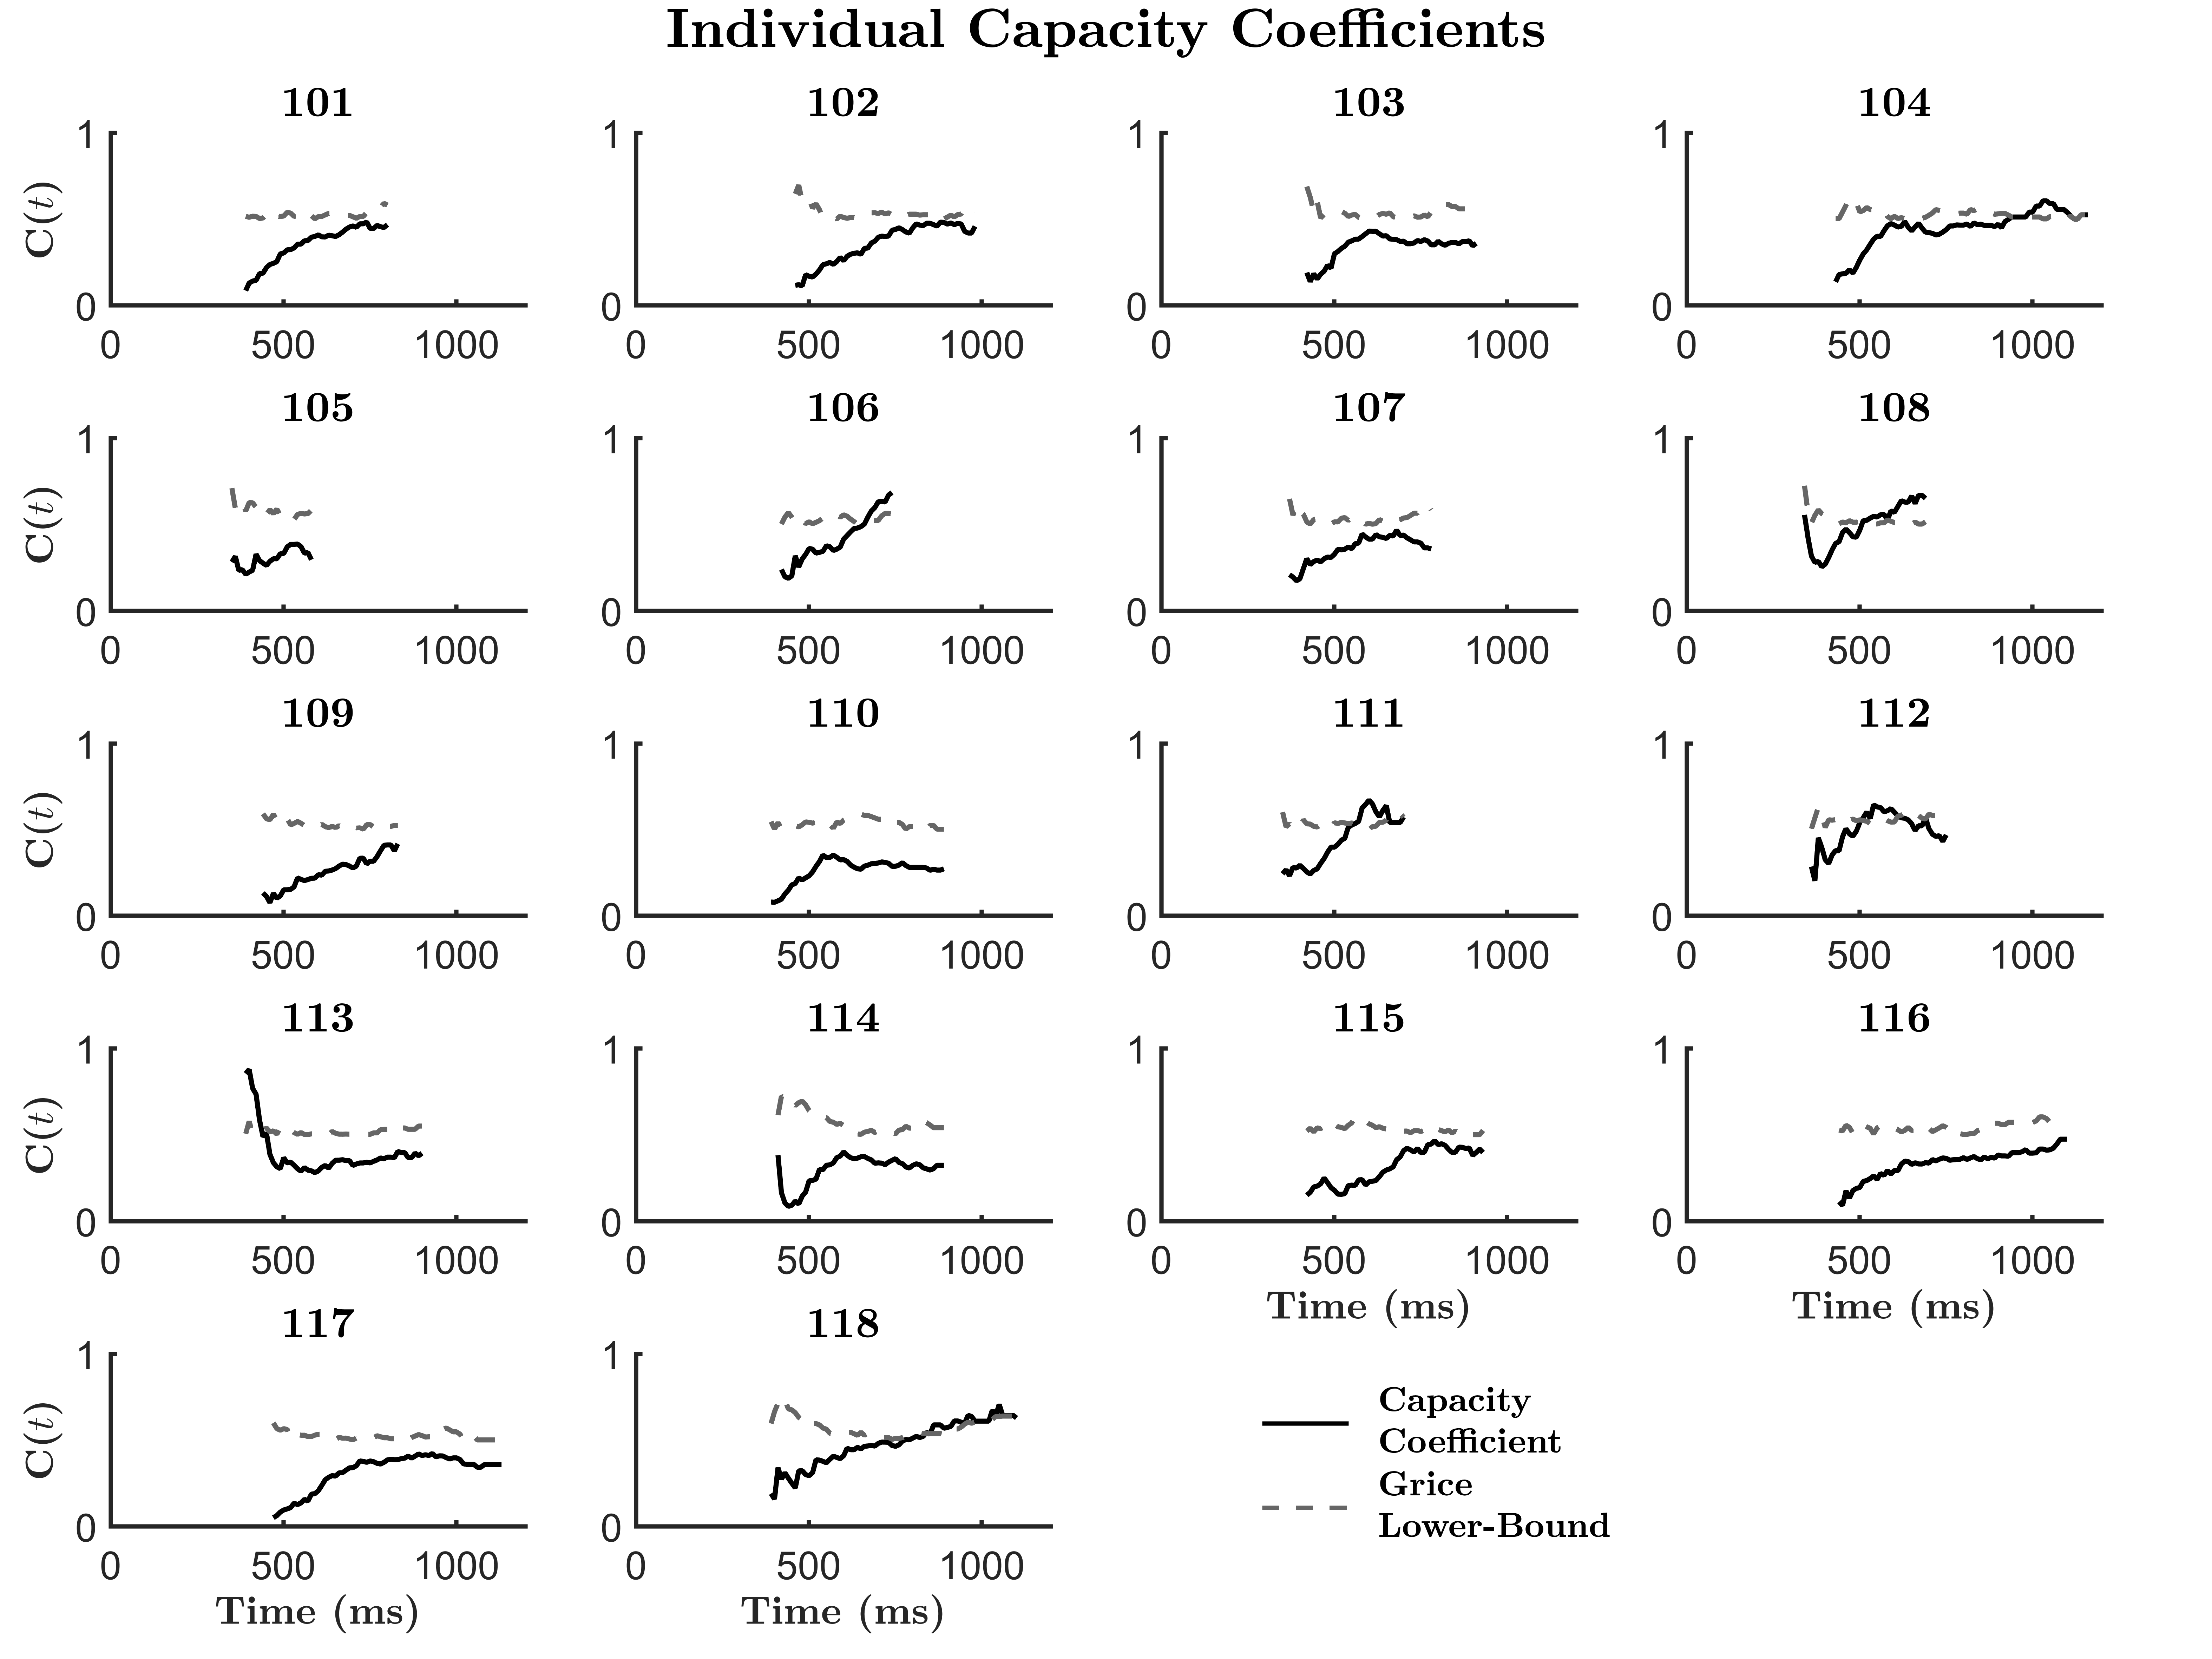
\includegraphics[width=\linewidth]{Figures/Appendix/FIG16JPG.jpg}
\caption{Capacity coefficient plots for each individual subject in Experiment 1. Dotted line depicts the Grice lower-bound. Black solid line illustrates the target capacity coefficient. All capacity coefficients are illustrated as on or below the lower-bound, suggesting severe workload capacity limitations in all subjects.}
\label{fig:Indiv_Cap_Ex1}
\end{center}
\end{figure}

\newpage
\subsection{Experiment 2: Fixed Item-Size, Spatially Separate Item-Sets}
\begin{figure}[htb]
\begin{center}
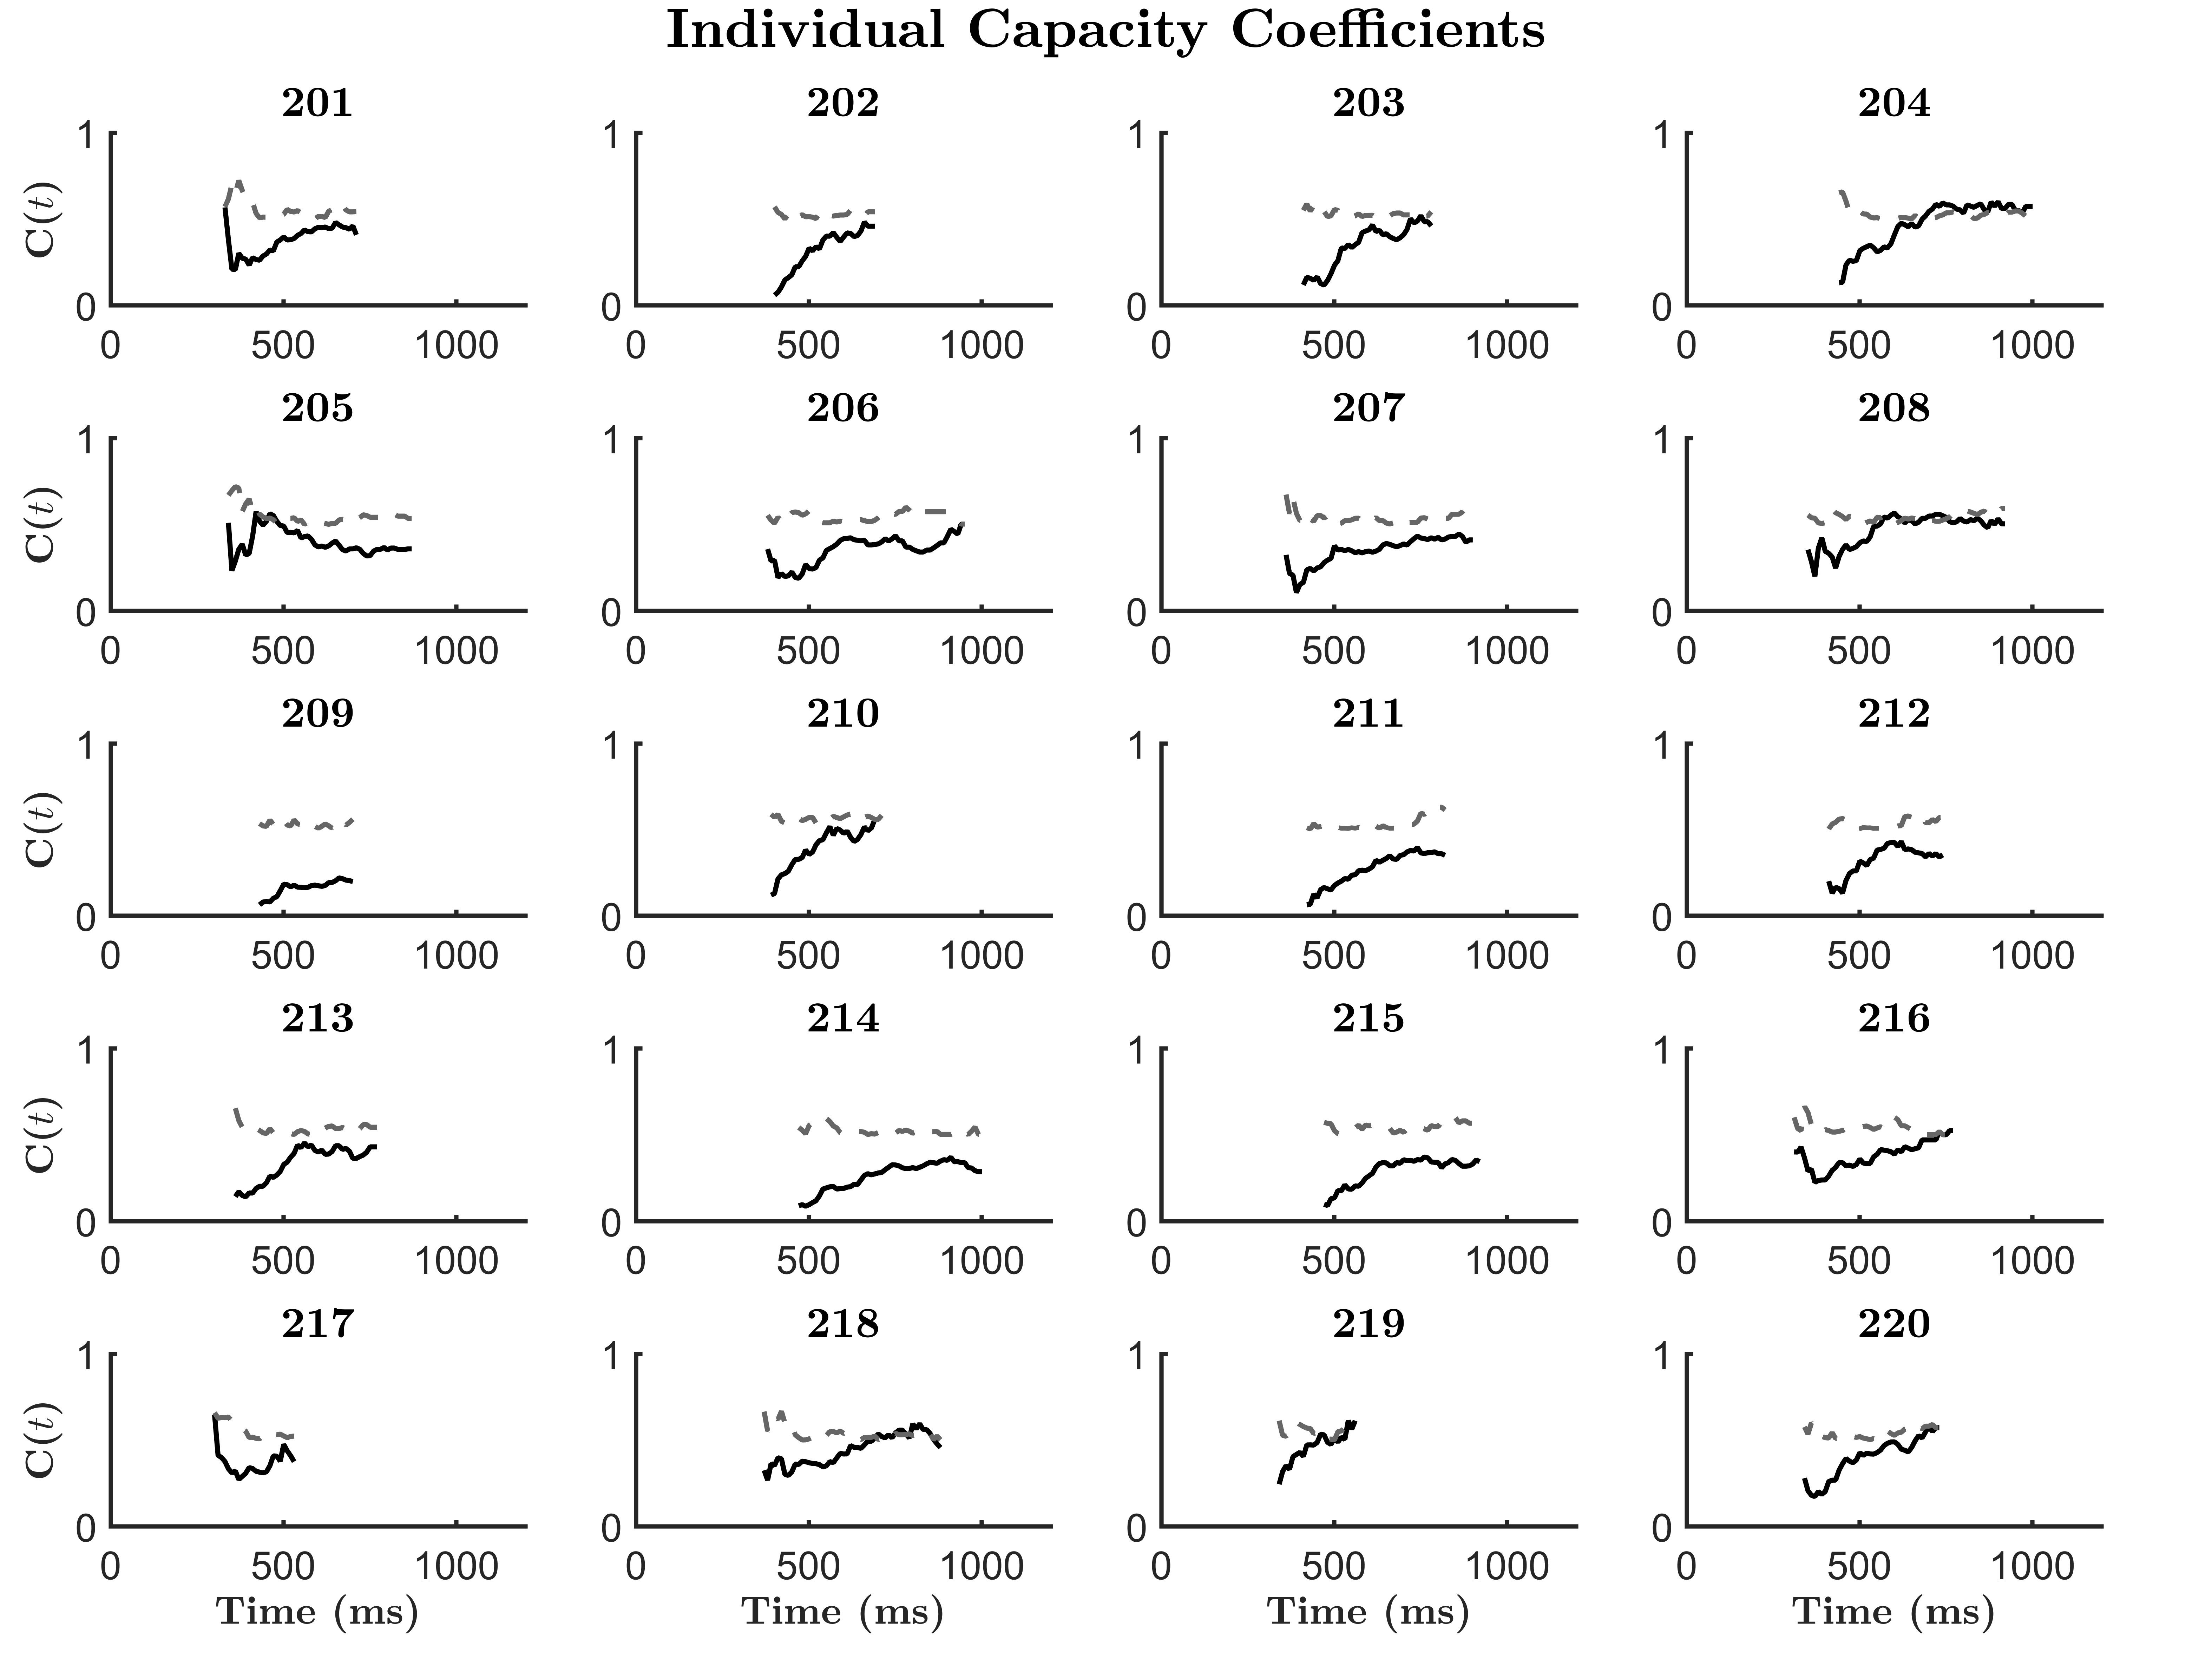
\includegraphics[width=\linewidth]{Figures/Appendix/FIG17JPG.jpg}
\caption{Capacity coefficient plots for each individual subject in Experiment 2. Dotted line depicts the Grice lower-bound. Black solid line illustrates the target capacity coefficient. All capacity coefficients are illustrated as on or below the lower-bound, suggesting severe workload capacity limitations in all subjects.}
\label{fig:Indiv_Cap_Ex2}
\end{center}
\end{figure}

\newpage
\subsection{Experiment 3: Fixed Item-Set Area, Mixed Item-Sets}
\begin{figure}[htb]
\begin{center}
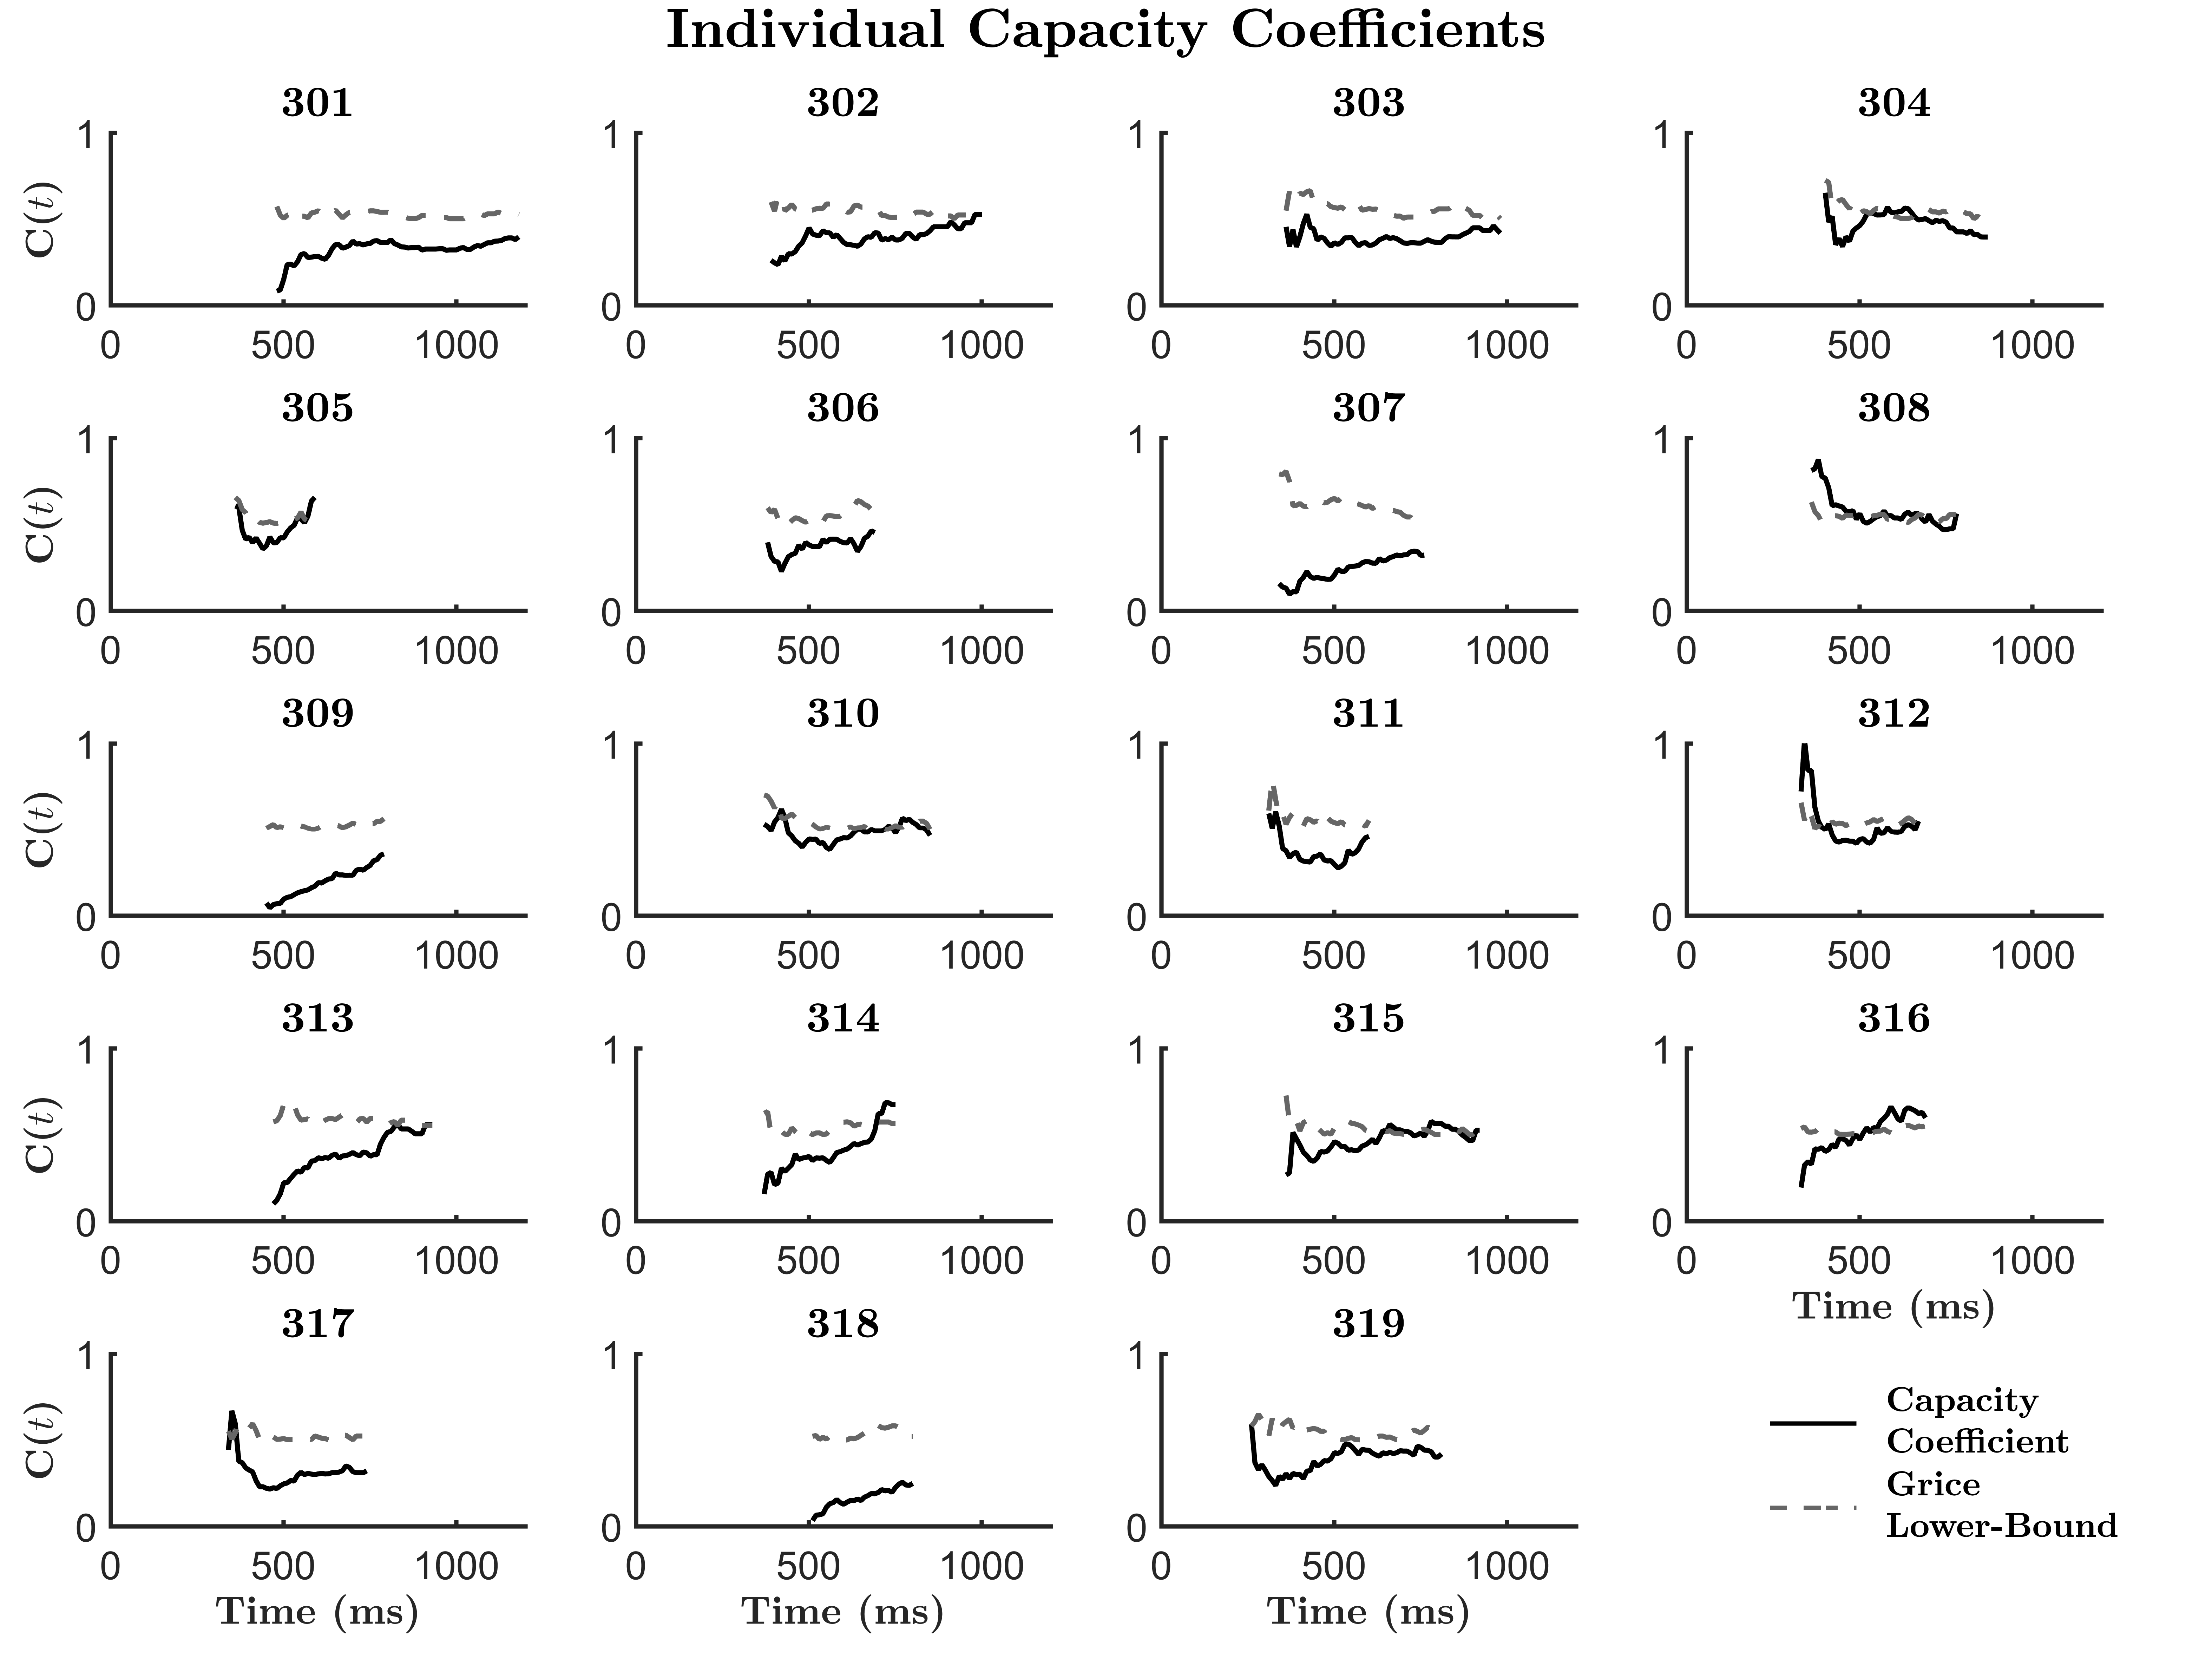
\includegraphics[width=\linewidth]{Figures/Appendix/FIG18JPG.jpg}
\caption{Capacity coefficient plots for each individual subject in Experiment 3. Dotted line depicts the Grice lower-bound. Black solid line illustrates the target capacity coefficient. All capacity coefficients are illustrated as on or below the lower-bound, suggesting severe workload capacity limitations in all subjects.}
\label{fig:Indiv_Cap_Ex3}
\end{center}
\end{figure}

\newpage
\subsection{Experiment 4: Fixed Item-Set Area, Spatially Separated Item-Sets}
\begin{figure}[htb]
\begin{center}
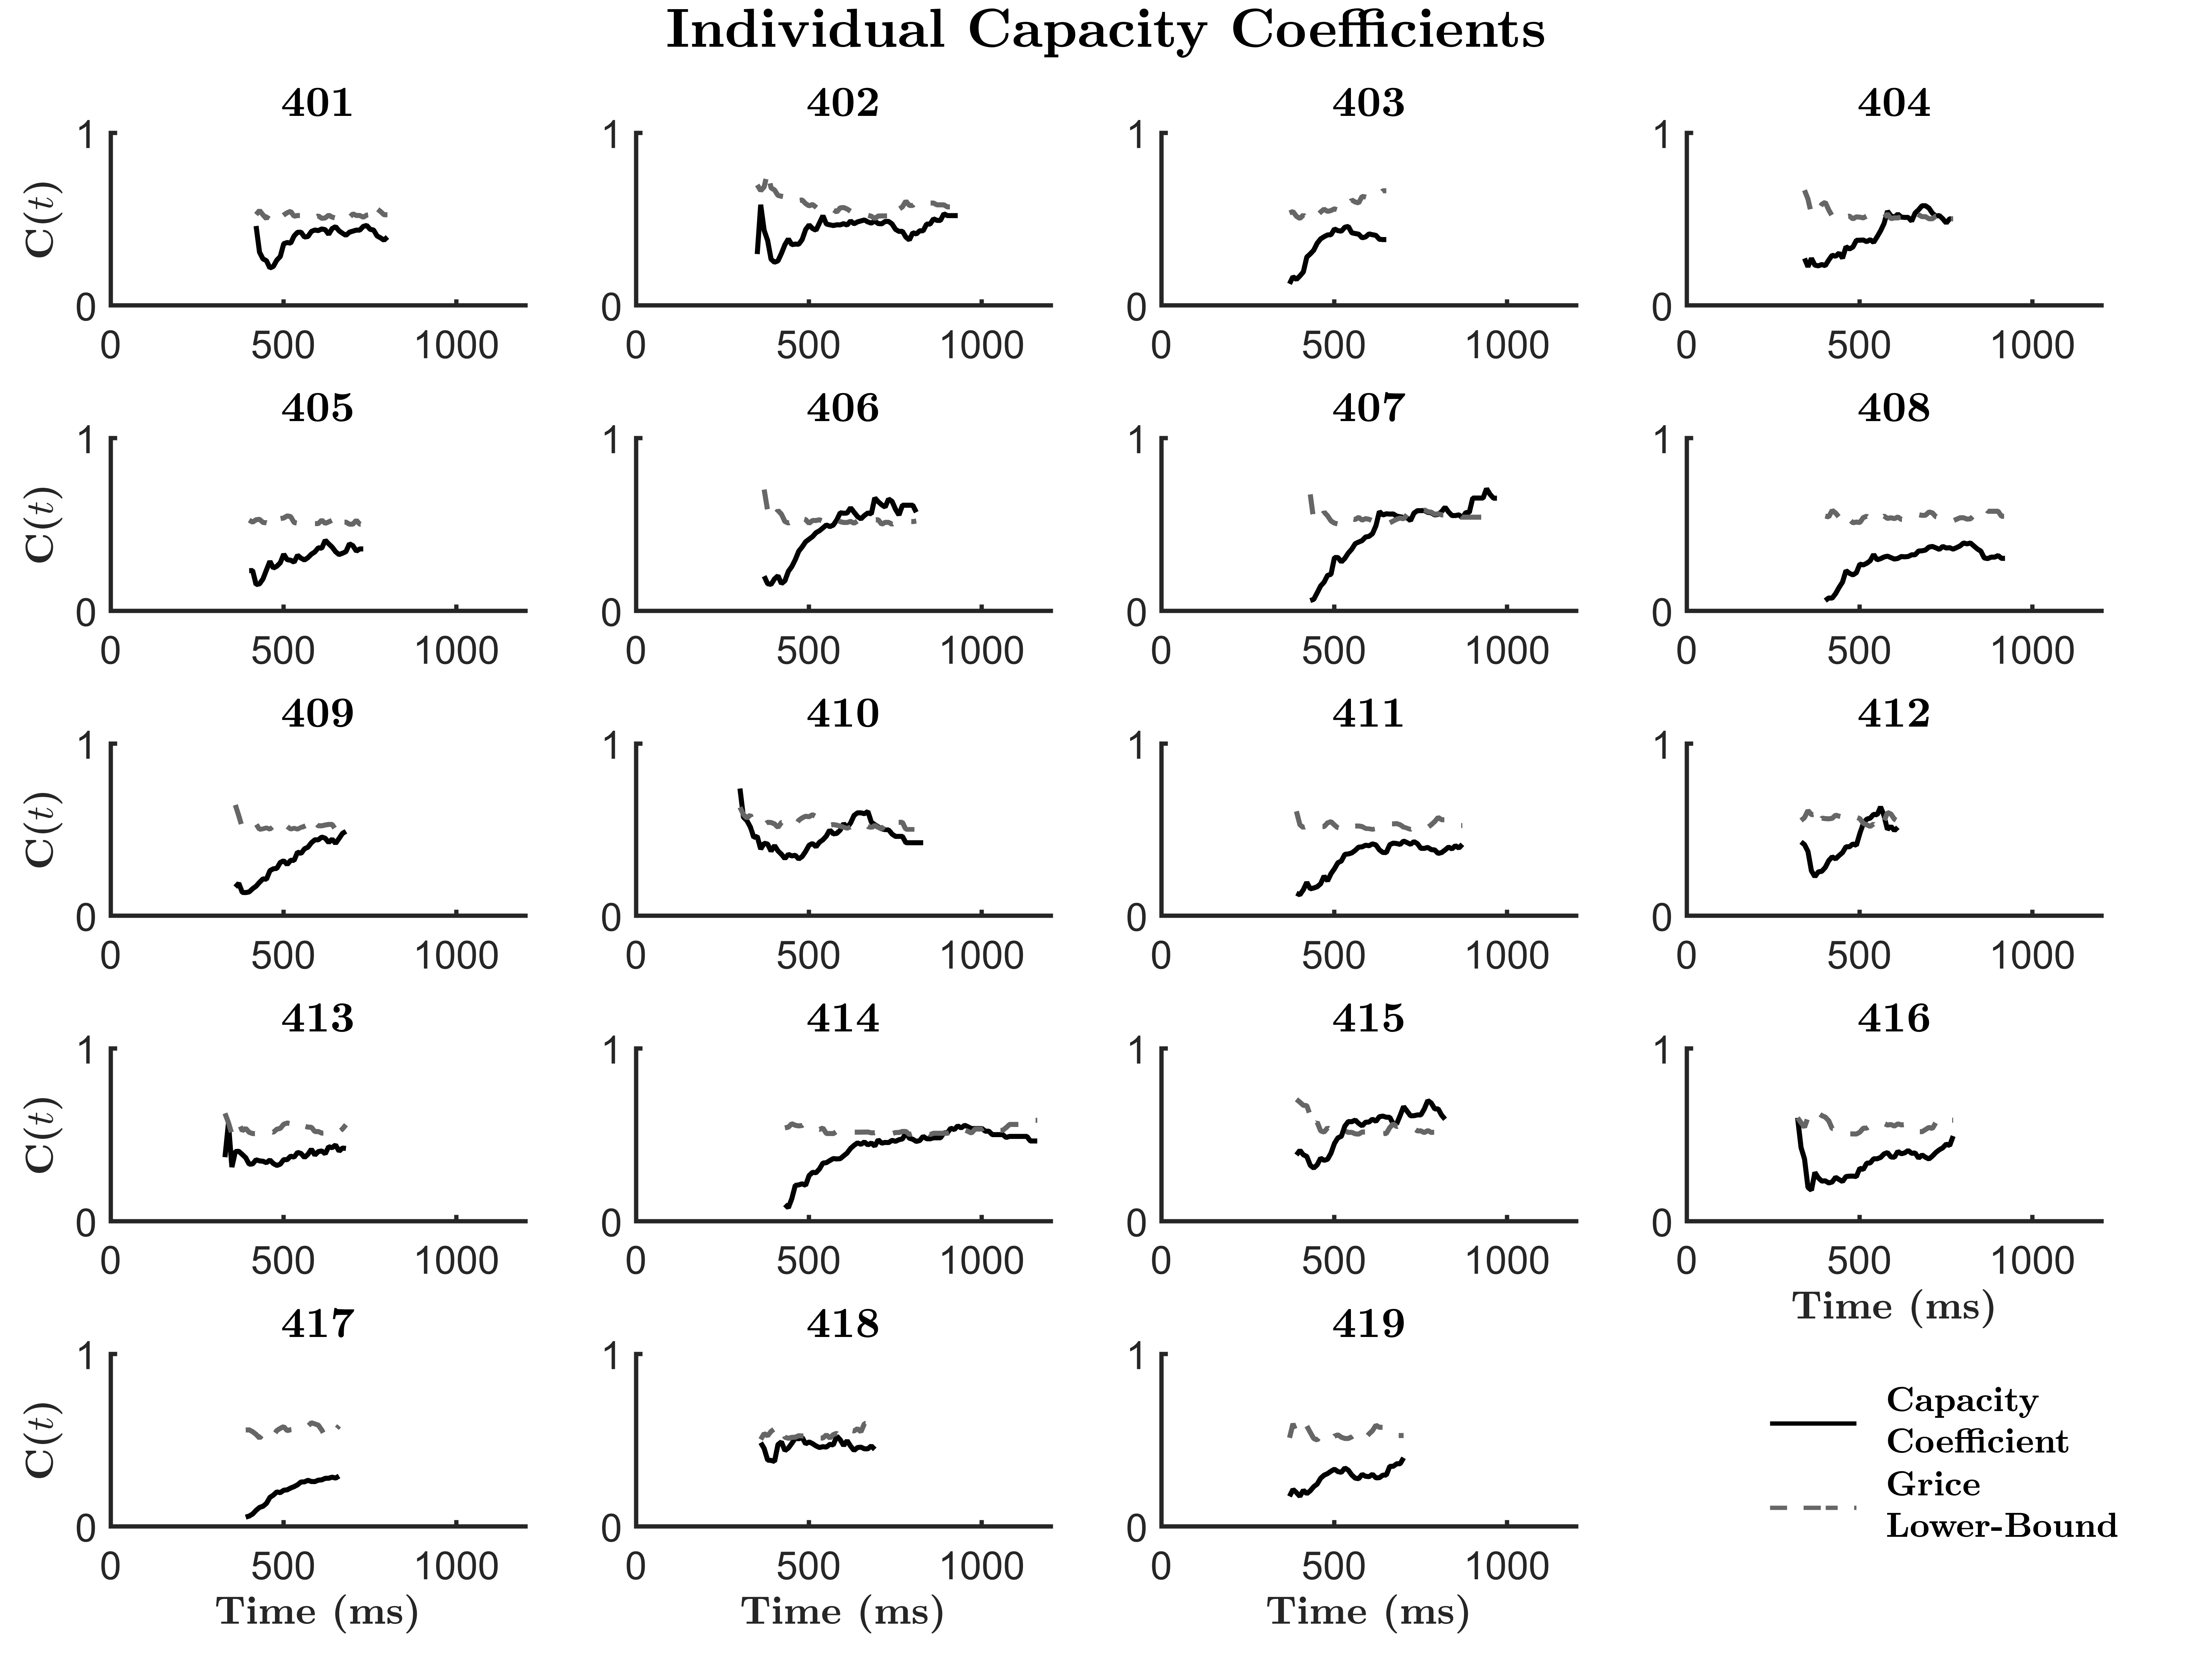
\includegraphics[width=\linewidth]{Figures/Appendix/FIG19JPG.jpg}
\caption{Capacity coefficient plots for each individual subject in Experiment 4. Dotted line depicts the Grice lower-bound. Black solid line illustrates the target capacity coefficient. All capacity coefficients are illustrated as on or below the lower-bound, suggesting severe workload capacity limitations in all subjects.}
\label{fig:Indiv_Cap_Ex4}
\end{center}
\end{figure}

\newpage
\section{Resilience Difference}
\label{Sup: Rdiff}

\begin{figure}[tbh]
\centering 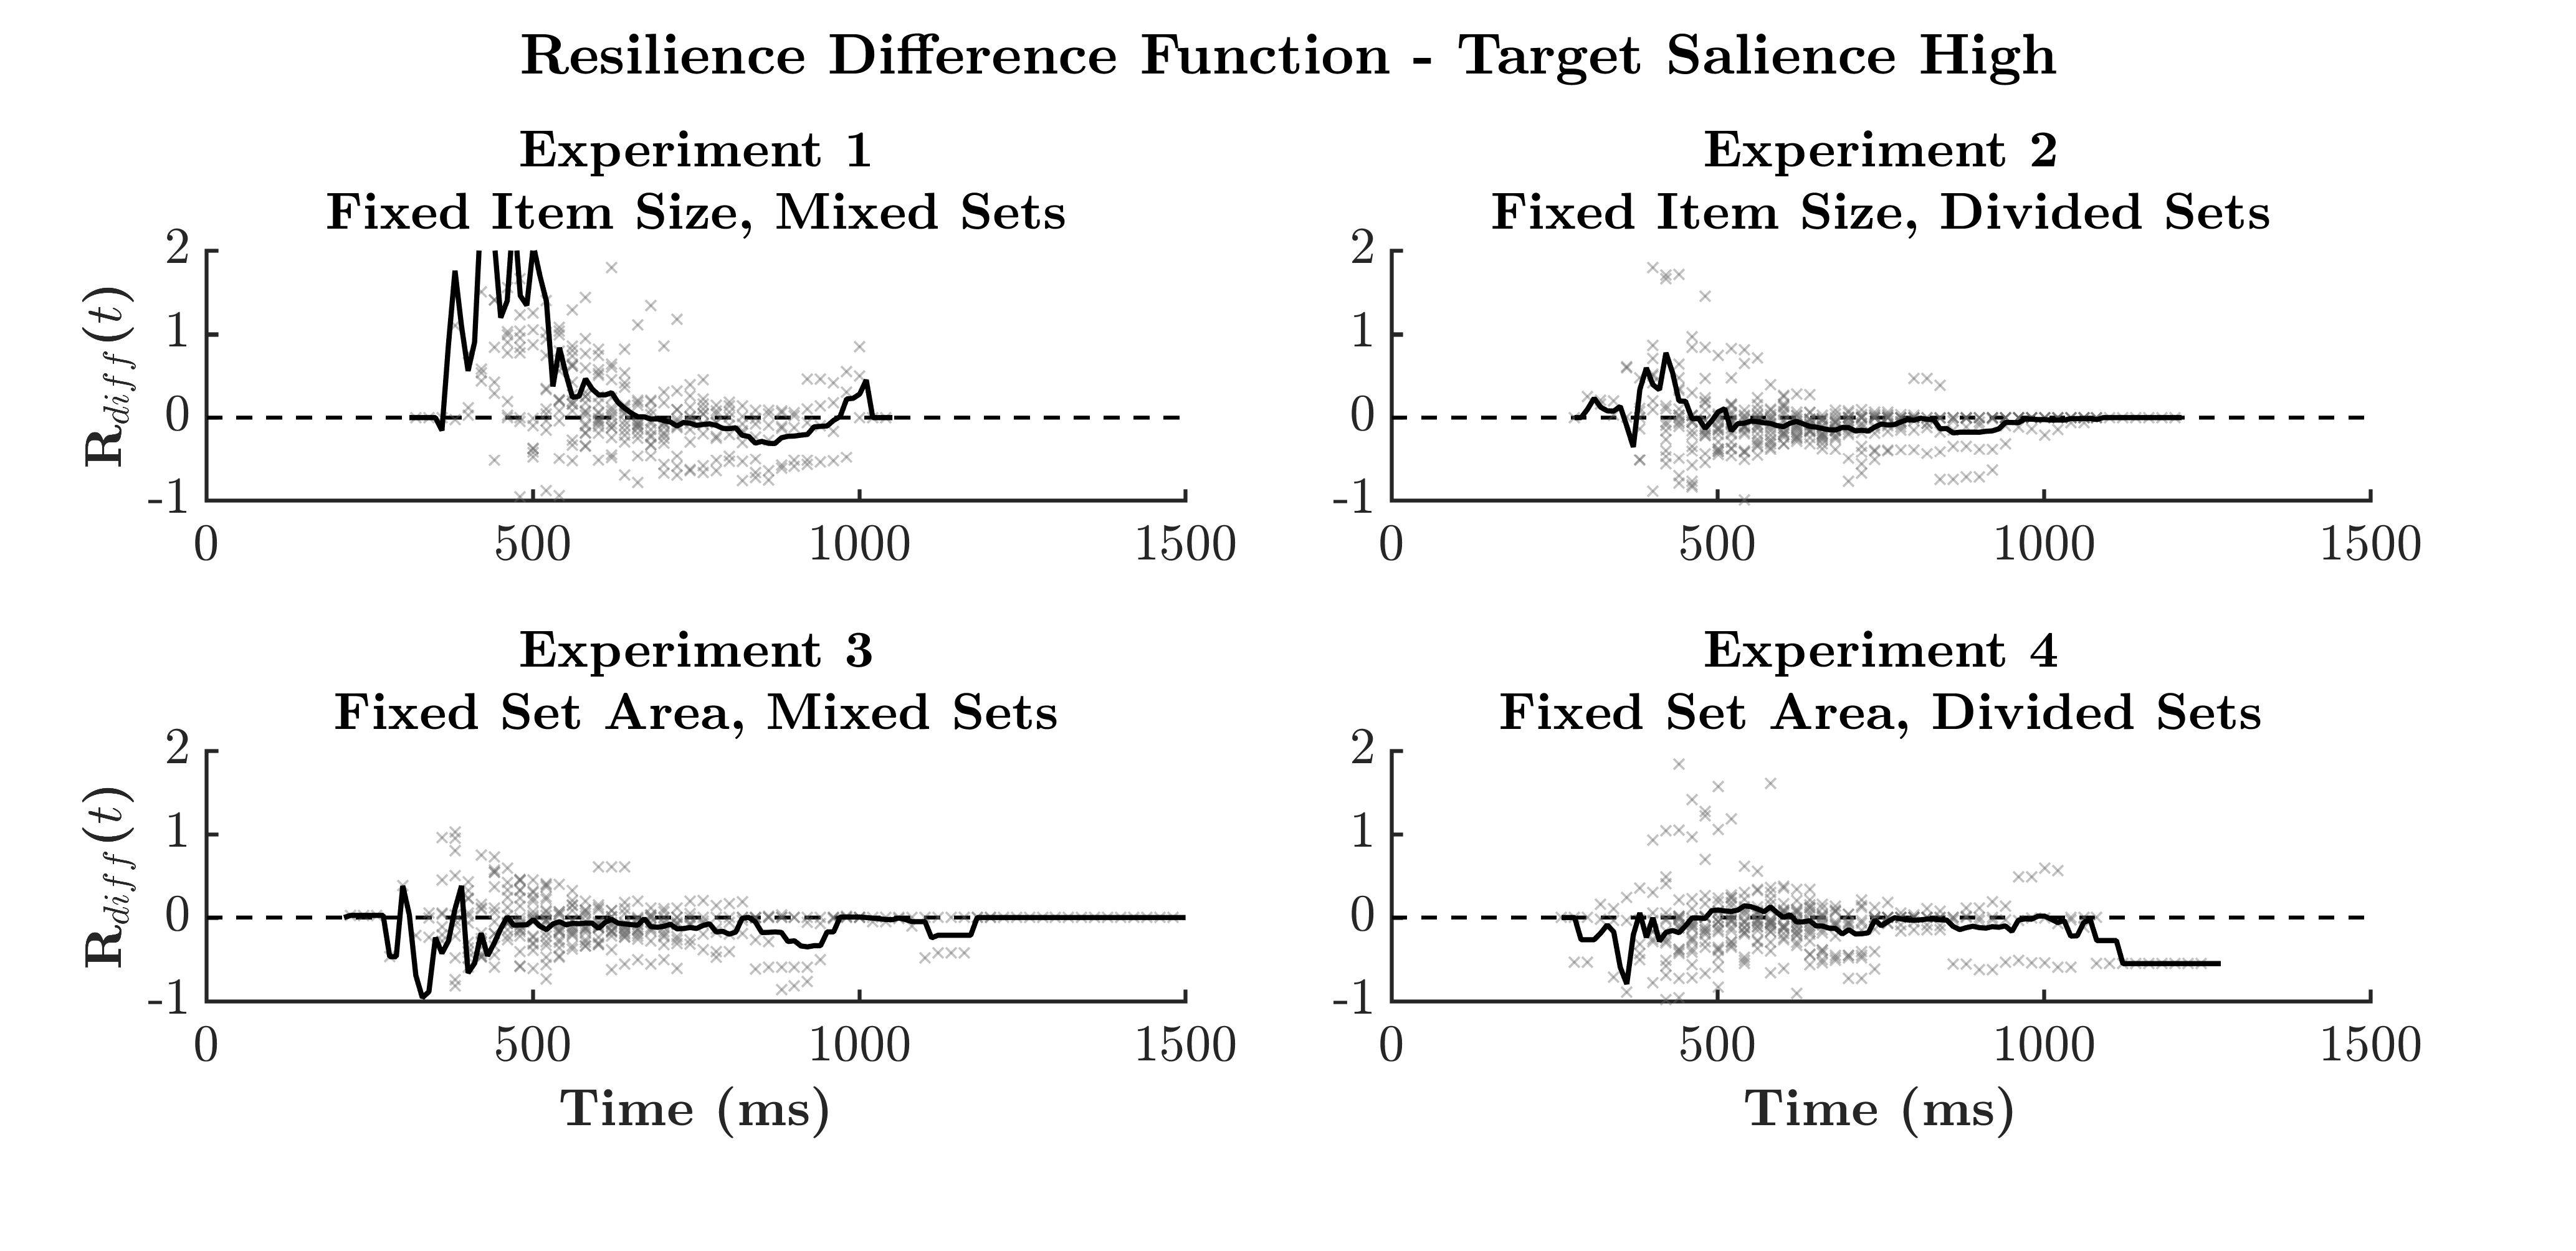
\includegraphics[width=\linewidth]{Figures/Appendix/FIG20JPG.jpeg}
\caption{Resilience difference plots for Estimation Experiments 1 – 4 when target salience is high. Black lines depict the average resilience difference function across subjects, while grey markers illustrate individual subject’s resilience difference functions. Average plots show a trend towards \Rd = 0, supporting predictions made by an unlimited-capacity parallel minimum-time processing system.}
\label{fig:RdiffHigh}
\end{figure}


\newpage
\section{Processing Architecture}
\label{Appendix: DT_Arch}
\subsection{Experiments 2--4}
\begin{table}[htb]
\caption{Table of individual double-target MIC and SIC results from Experiments 2--4. From left to right, ANOVA main effects for red target salience (R) and blue target salience (B), MIC value and interaction significance, Bayesian SIC model probability and associated architecture, and Bayes factor values from the hierarchical MIC analysis with associated processing architecture results: Parallel (P) and Serial (S).}
\centering 
\begin{tabular*}{\textwidth}{l @{\extracolsep{\fill}} lllllll}
\hhline{-------}
\textbf{Sub  } & \textbf{\begin{tabular}[c]{@{}c@{}}Main \\ Effects\end{tabular}} & \textbf{MIC} & \textbf{SIC} $\mathbb{P}$ & \textbf{SIC Model} & \textbf{BF$_{10}$} & \textbf{MIC Model} \\  
\hhline{-------}
202 & R \& B & 30*   &\textbf{0.57}& \textbf{P Min-Time}  & \textbf{4.6}  & \textbf{P Min-Time}\\
205 & R \& B & 112*  & &                                  & \textbf{15.32} & \textbf{P Min-Time}\\
212 & R \& B & 8     &0.44         & P Min-Time           & \textbf{3.18}  & \textbf{P Min-Time}\\
214 & R \& B & 142** &\textbf{0.95}& \textbf{P Min-Time}  & \textbf{18.75} & \textbf{P Min-Time}\\
215 & R \& B & 78* 	 &\textbf{0.67}& \textbf{P Min-Time}  & \textbf{10.42}  & \textbf{P Min-Time}\\
\hhline{~~~~---}
~&~&~&~& \textit{MIC Group Posterior}                              & \textbf{5.11}  & \textbf{P Min-Time} \\       
\hhline{-------}
303 & R \& B & 128** &\textbf{0.95}& \textbf{P Min-Time}  & \textbf{13.95} & \textbf{P Min-Time}\\ 
307 & R \& B & -7    &0.41& P Min-Time                    & 2.27 & P Min-Time\\      
310 & R \& B & 26    &\textbf{0.64}& \textbf{P Min-Time}  & \textbf{3.35} & \textbf{P Min-Time}\\      
311 & R \& B & 13    &&                                   & 2.44 & P Min-Time\\
318 & R \& B & 67* 	 &\textbf{0.69}& \textbf{P Min-Time}  & \textbf{6.9} & \textbf{P Min-Time}\\ 
\hhline{~~~~---}
~&~&~&~& \textit{MIC Group Posterior}                              & \textbf{3.42} & \textbf{P Min-Time} \\ 
\hhline{-------}
402 & R \& B & -45*  &\textbf{0.65}& \textbf{P Max-Time}  & 1.9   & P Max-Time\\     
407 & R \& B & 72**  &\textbf{0.64}& \textbf{P Min-Time}  & \textbf{8.73}  & \textbf{P Min-Time}\\ 
414 & R \& B & 116** &&                                   & \textbf{12.42} & \textbf{P Min-Time}\\         
416 & R \& B & -54*  &\textbf{0.91}& \textbf{P Max-Time}  & 2.68  & P Max-Time\\ 
\hhline{~~~~---}
~&~&~&~& \textit{MIC Group Posterior} & 2.68 & P Min-Time \\
\hhline{-------} \hhline{-------}
\multicolumn{7}{p{\textwidth}}{MIC interaction significance tests were conducted at p $<$ .33*, p $<$ .05** and p $<$ .01***. Conclusive model architectures were based upon an SIC model selection probability $>$ 0.5 and are displayed in bold font. MIC models with moderate evidence (BF$_{10}$ $>$ 3) are also displayed in bold font.}
\end{tabular*} 
\label{table:DT} 
\end{table}

\newpage

\label{Sup: indSIC}
\subsection{Experiment 1: Fixed Item-Size, Mixed Item-Sets Double-Target SIC}
\begin{figure}[htb]
\begin{center}
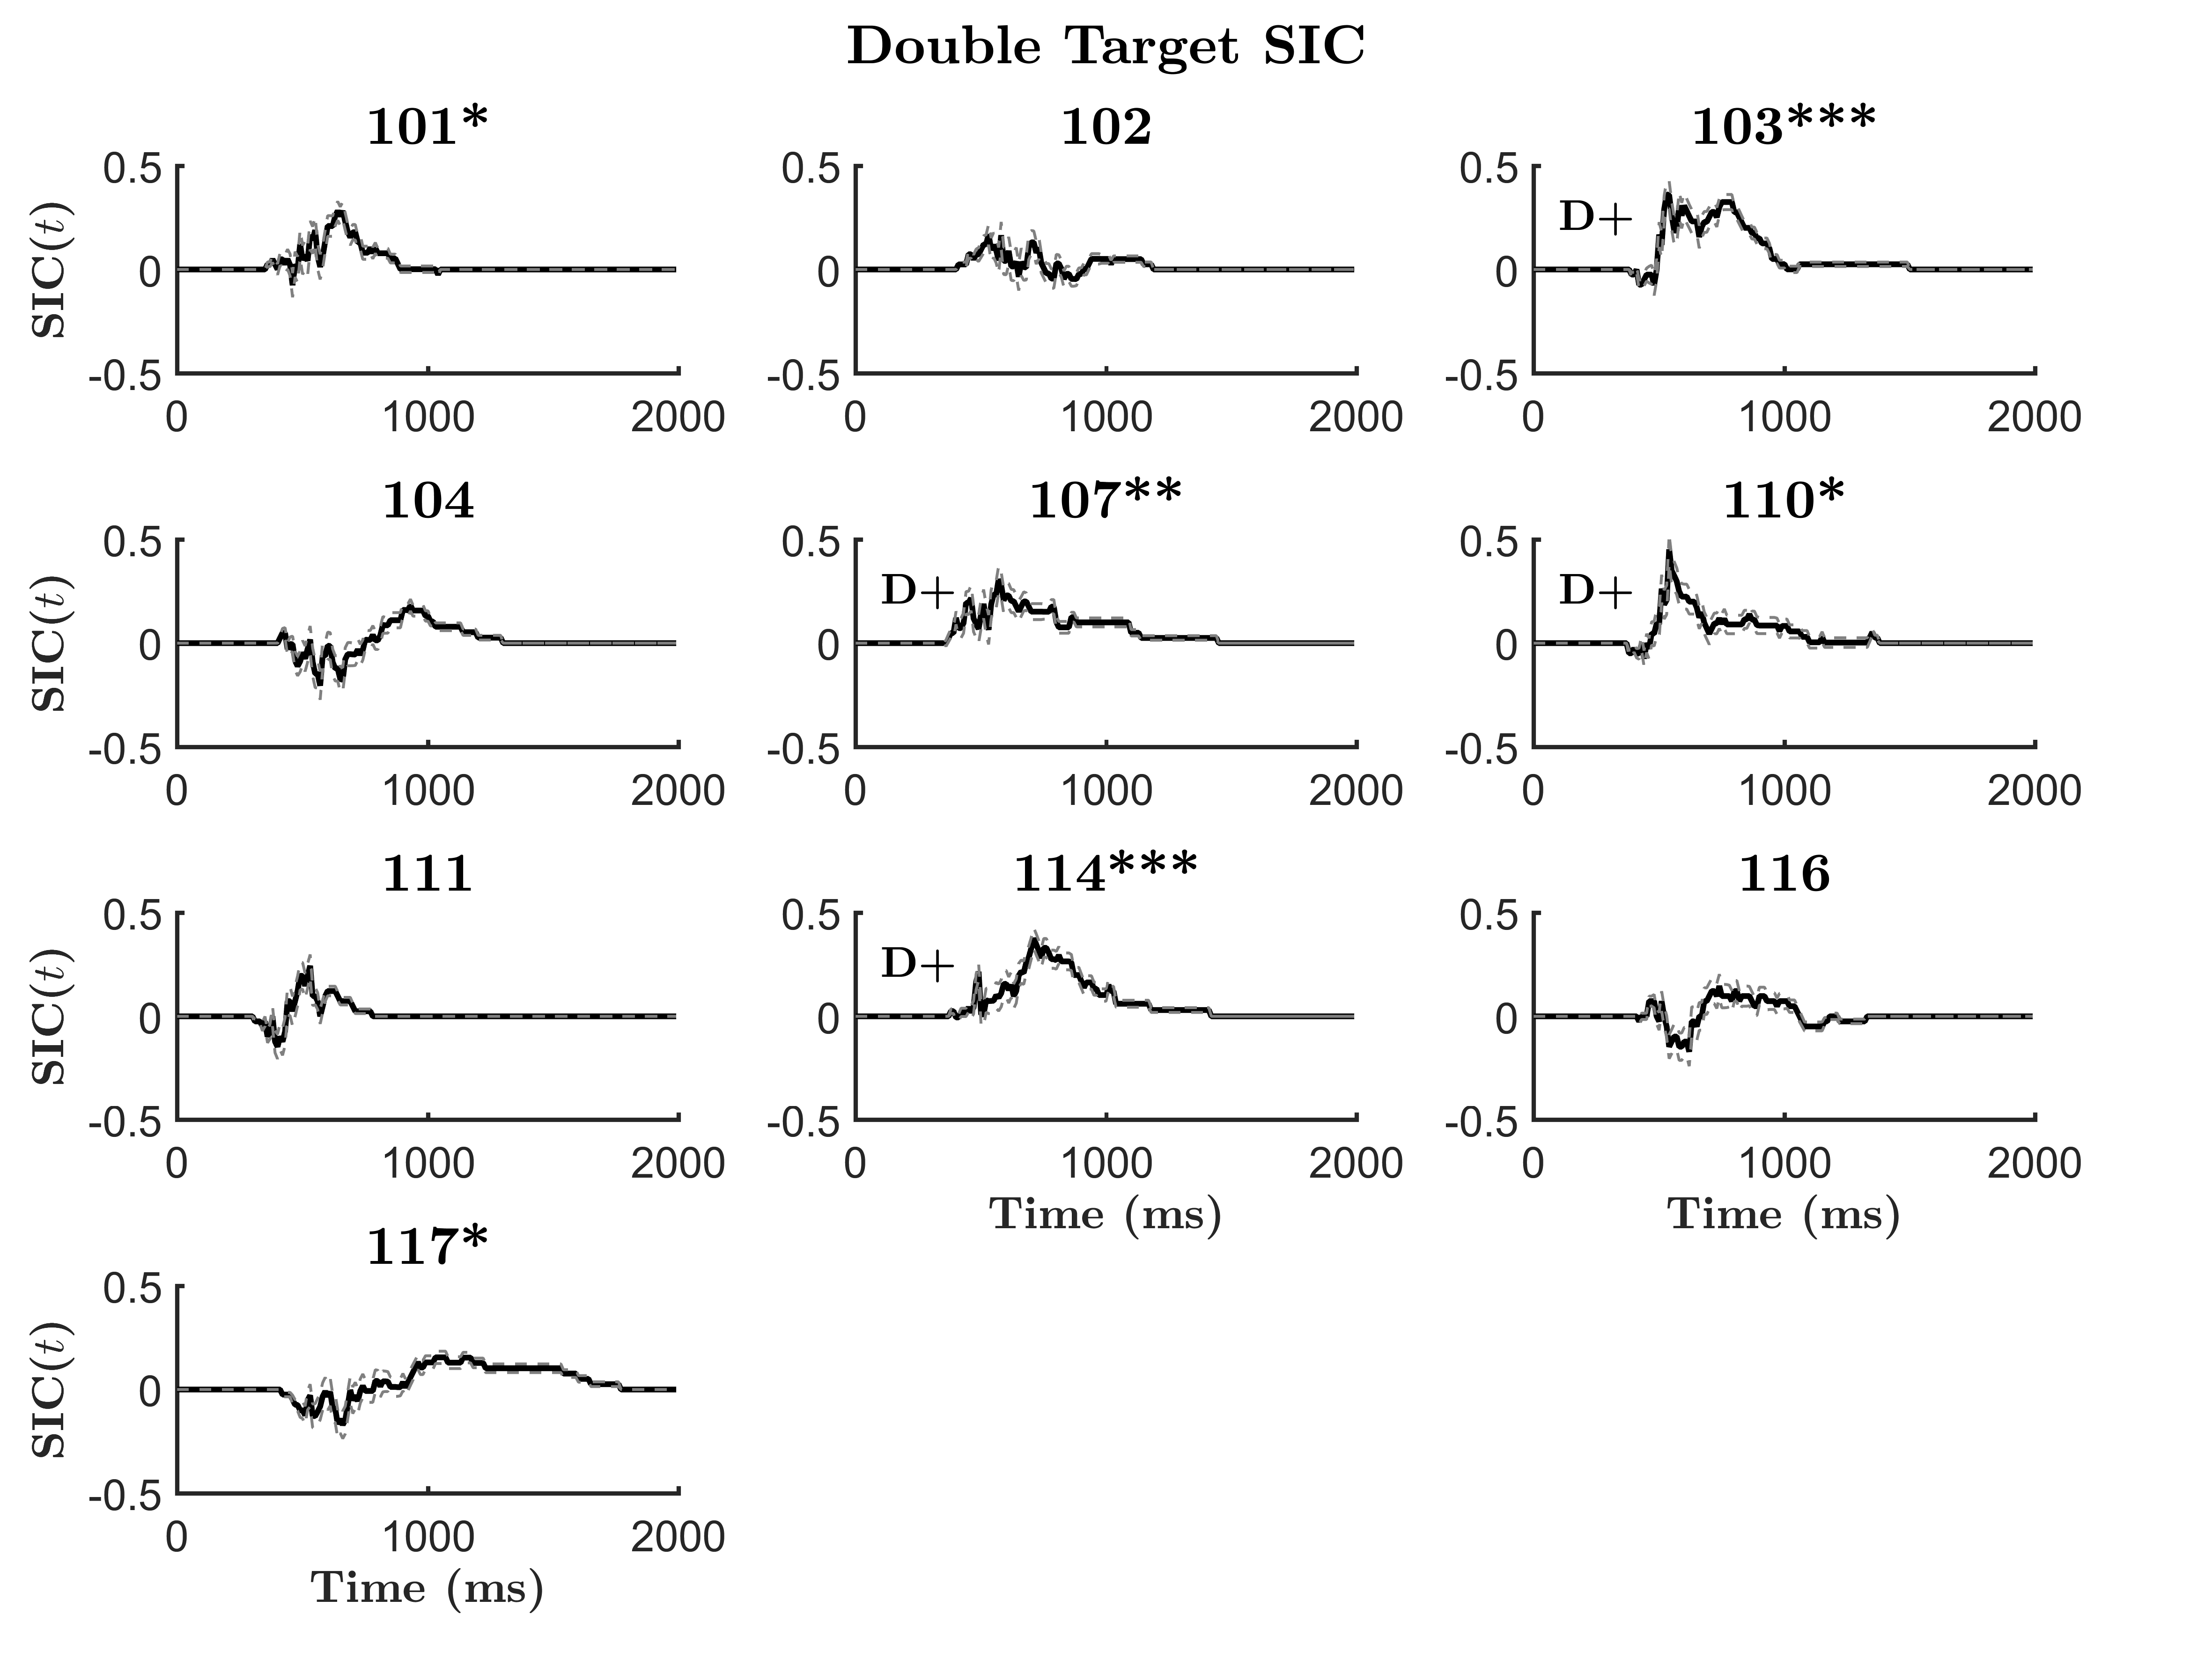
\includegraphics[width=\linewidth]{Figures/Appendix/FIG23PNG.png}
\caption{Double-Target survivor interaction contrast (SIC) plots for each individual subject in Experiment 1. Dotted line illustrates the bootstrap of the standard error.\newline
\textbf{Note.} MIC interaction contrast significance defined at $p$* $<$ .33, $p$** $<$ .05, $p$*** $<$ .01. D-statistic, a measure of SIC deviance from SIC($t$) = 0 significance defined at $\alpha$ $<$ 0.15.}
\label{fig:Indiv_SIC_AB_Ex1}
\end{center}
\end{figure}
\newpage

\subsection{Experiment 2: Fixed Item-Size, Mixed Item-Sets Double-Target SIC}
\begin{figure}[htb]
\begin{center}
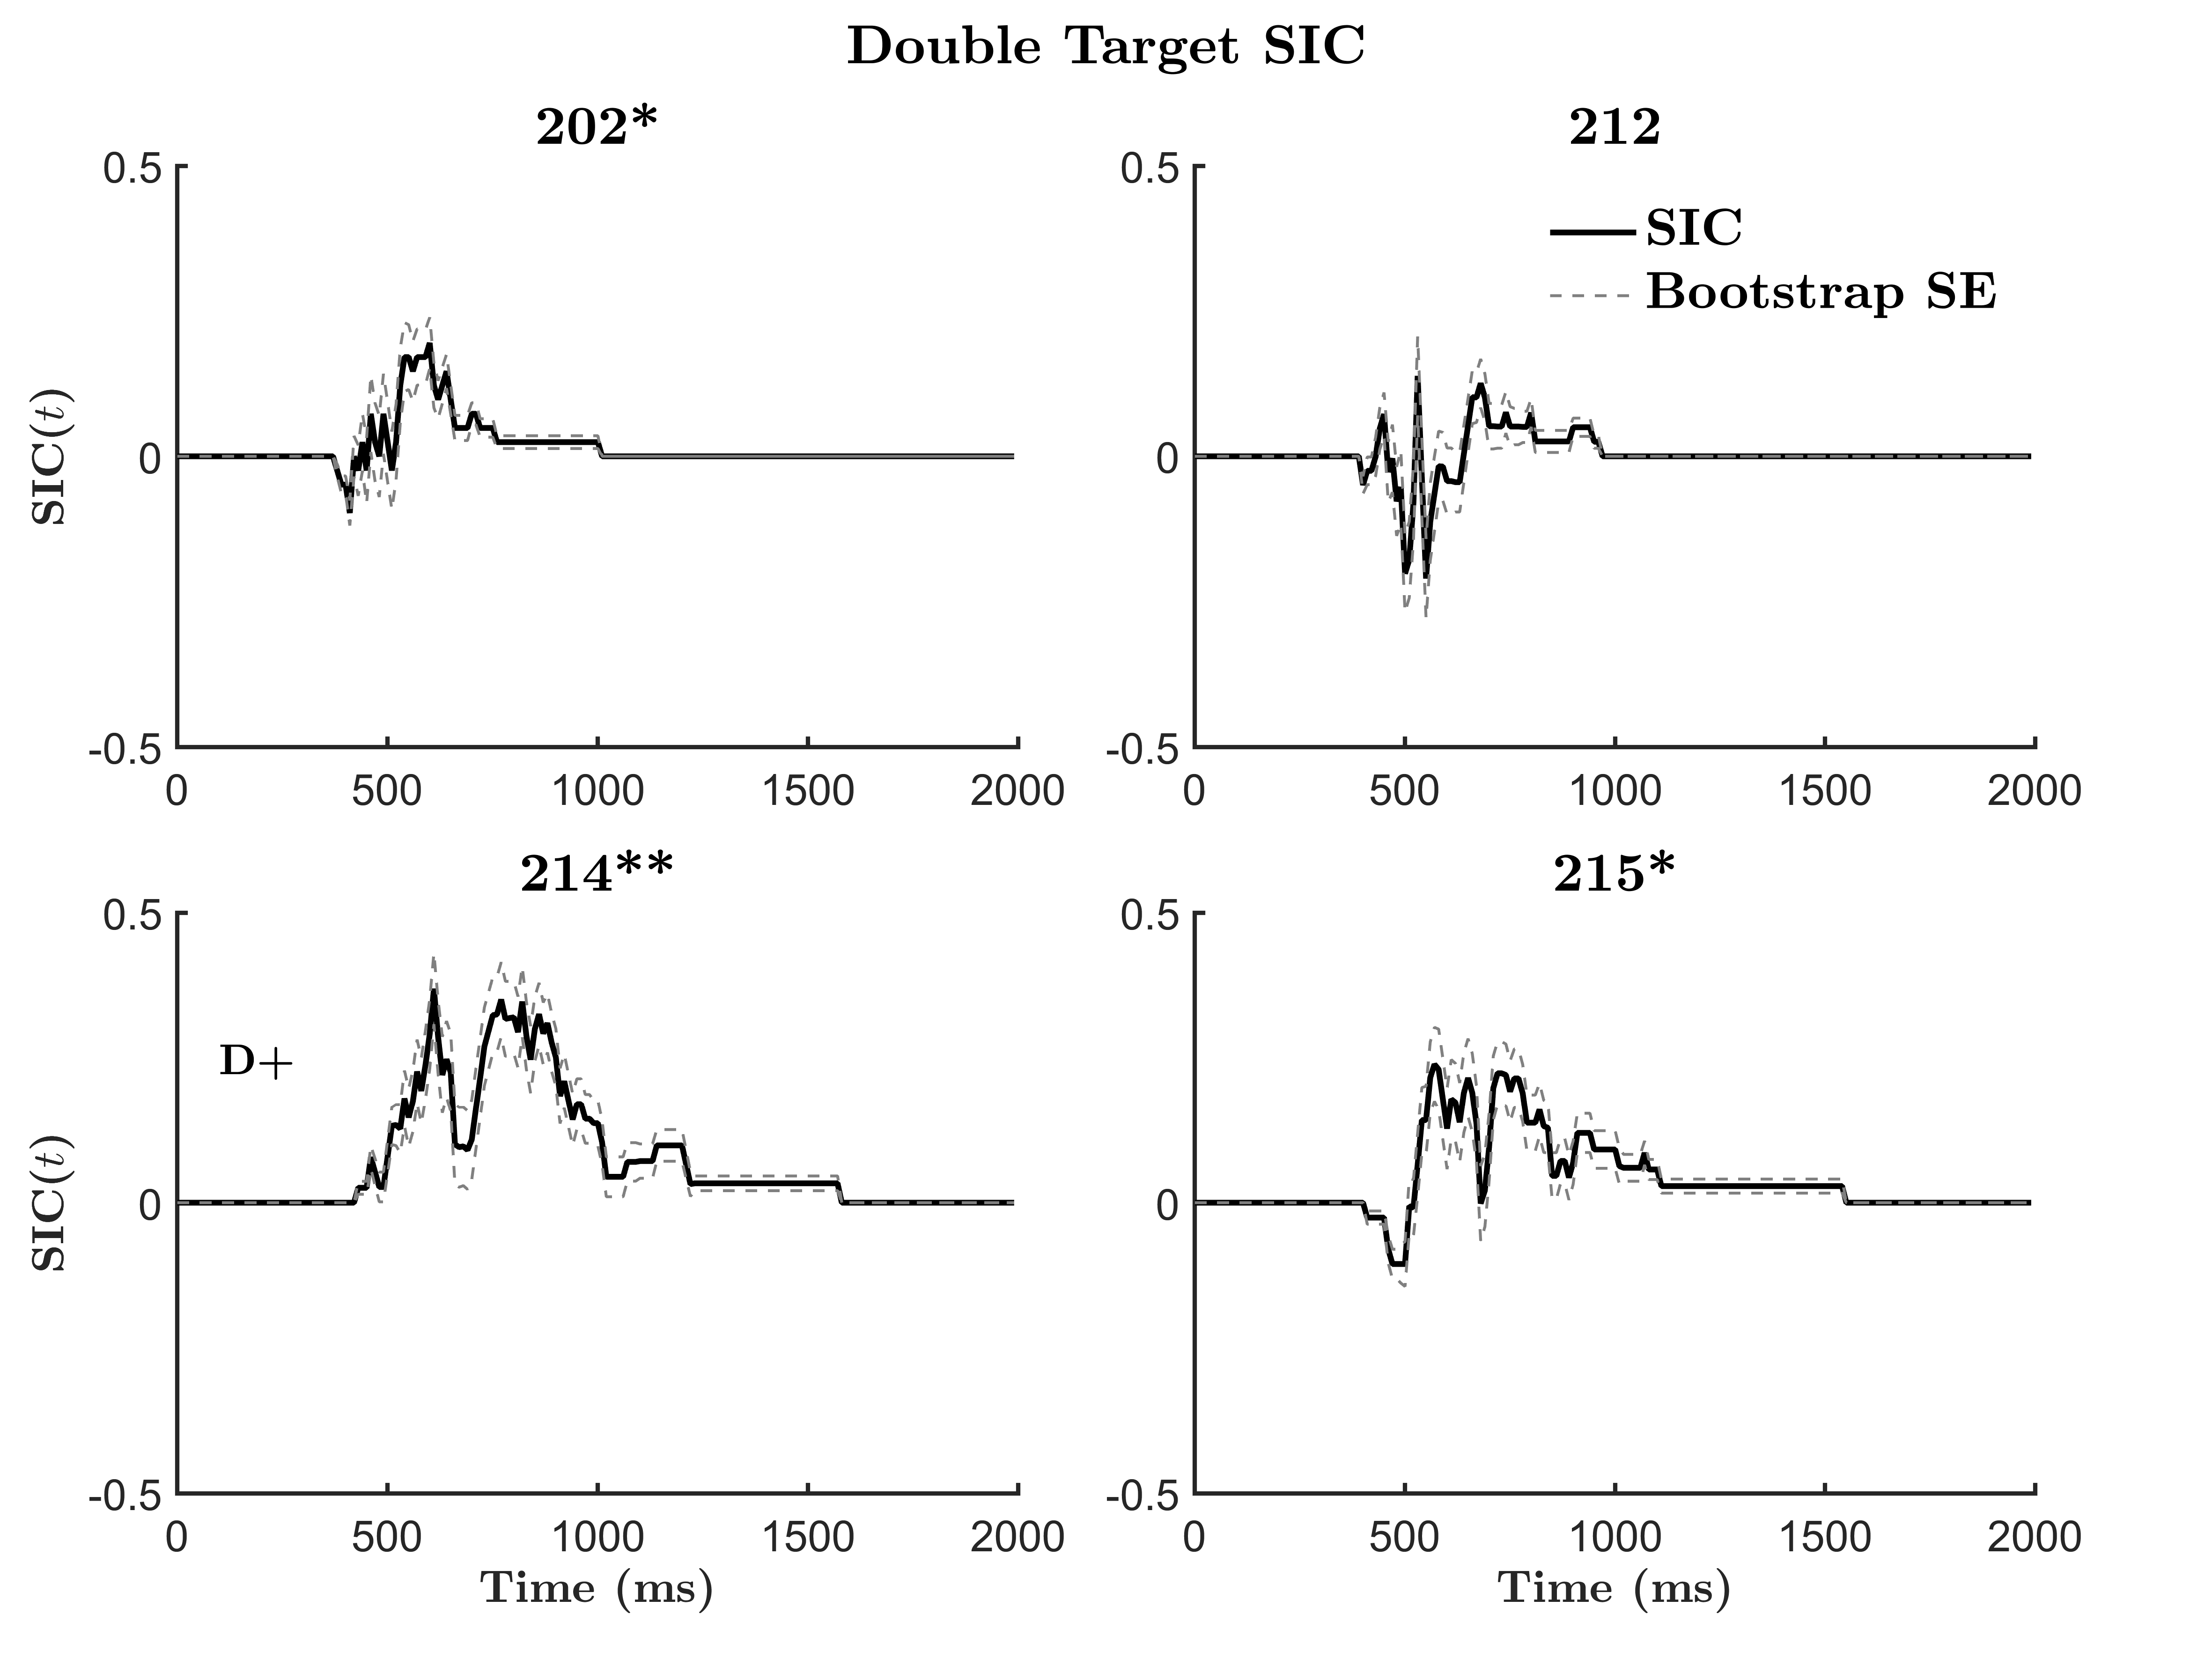
\includegraphics[width=\linewidth]{Figures/Appendix/FIG24PNG.png}
\caption{Double-Target survivor interaction contrast (SIC) plots for each individual subject in Experiment 2. Dotted line illustrates the bootstrap of the standard error.\newline
\textbf{Note.} MIC interaction contrast significance defined at $p$* $<$ .33, $p$** $<$ .05, $p$*** $<$ .01. D-statistic, a measure of SIC deviance from SIC($t$) = 0 significance defined at $\alpha$ $<$ 0.15.}
\label{fig:Indiv_SIC_AB_Ex2}
\end{center}
\end{figure}
\newpage

\subsection{Experiment 3: Fixed Item-Size, Mixed Item-Sets Double-Target SIC}
\begin{figure}[htb]
\begin{center}
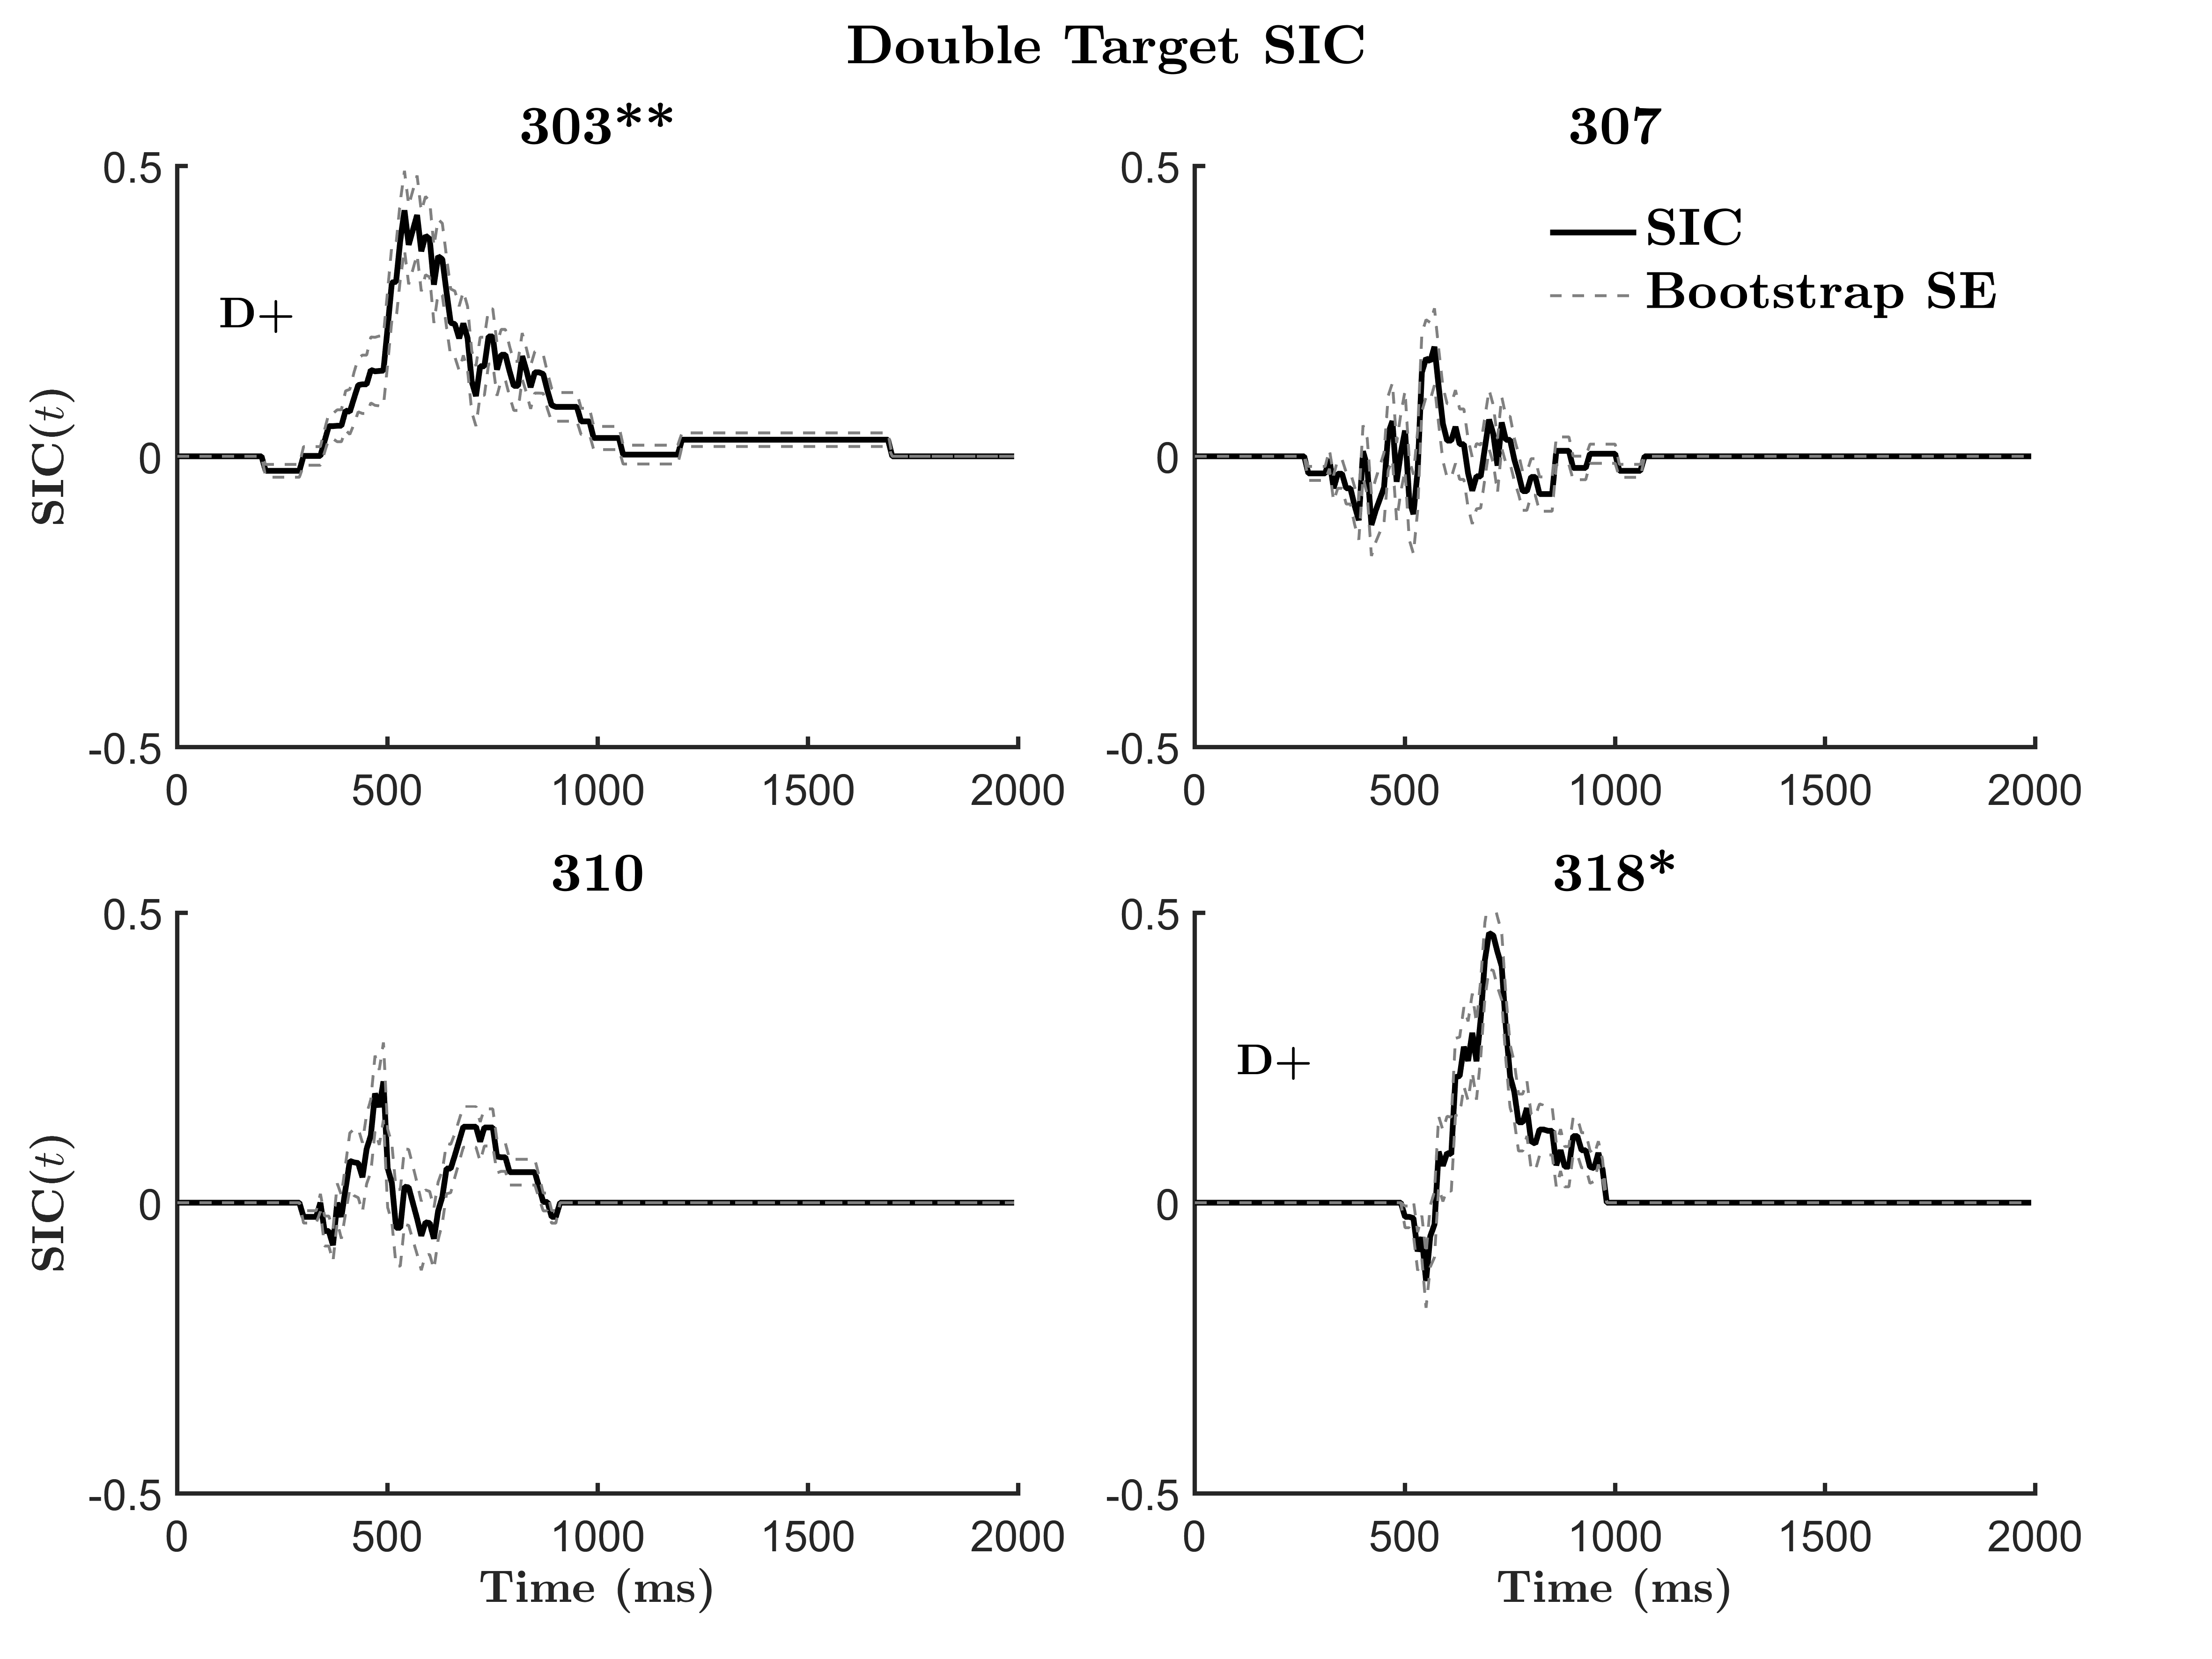
\includegraphics[width=\linewidth]{Figures/Appendix/FIG25PNG.png}
\caption{Double-Target survivor interaction contrast (SIC) plots for each individual subject in Experiment 3. Dotted line illustrates the bootstrap of the standard error.\newline
\textbf{Note.} MIC interaction contrast significance defined at $p$* $<$ .33, $p$** $<$ .05, $p$*** $<$ .01. D-statistic, a measure of SIC deviance from SIC($t$) = 0 significance defined at $\alpha$ $<$ 0.15.}
\label{fig:Indiv_SIC_AB_Ex3}
\end{center}
\end{figure}
\newpage

\subsection{Experiment 4: Fixed Item-Size, Mixed Item-Sets Double-Target SIC}
\begin{figure}[htb]
\begin{center}
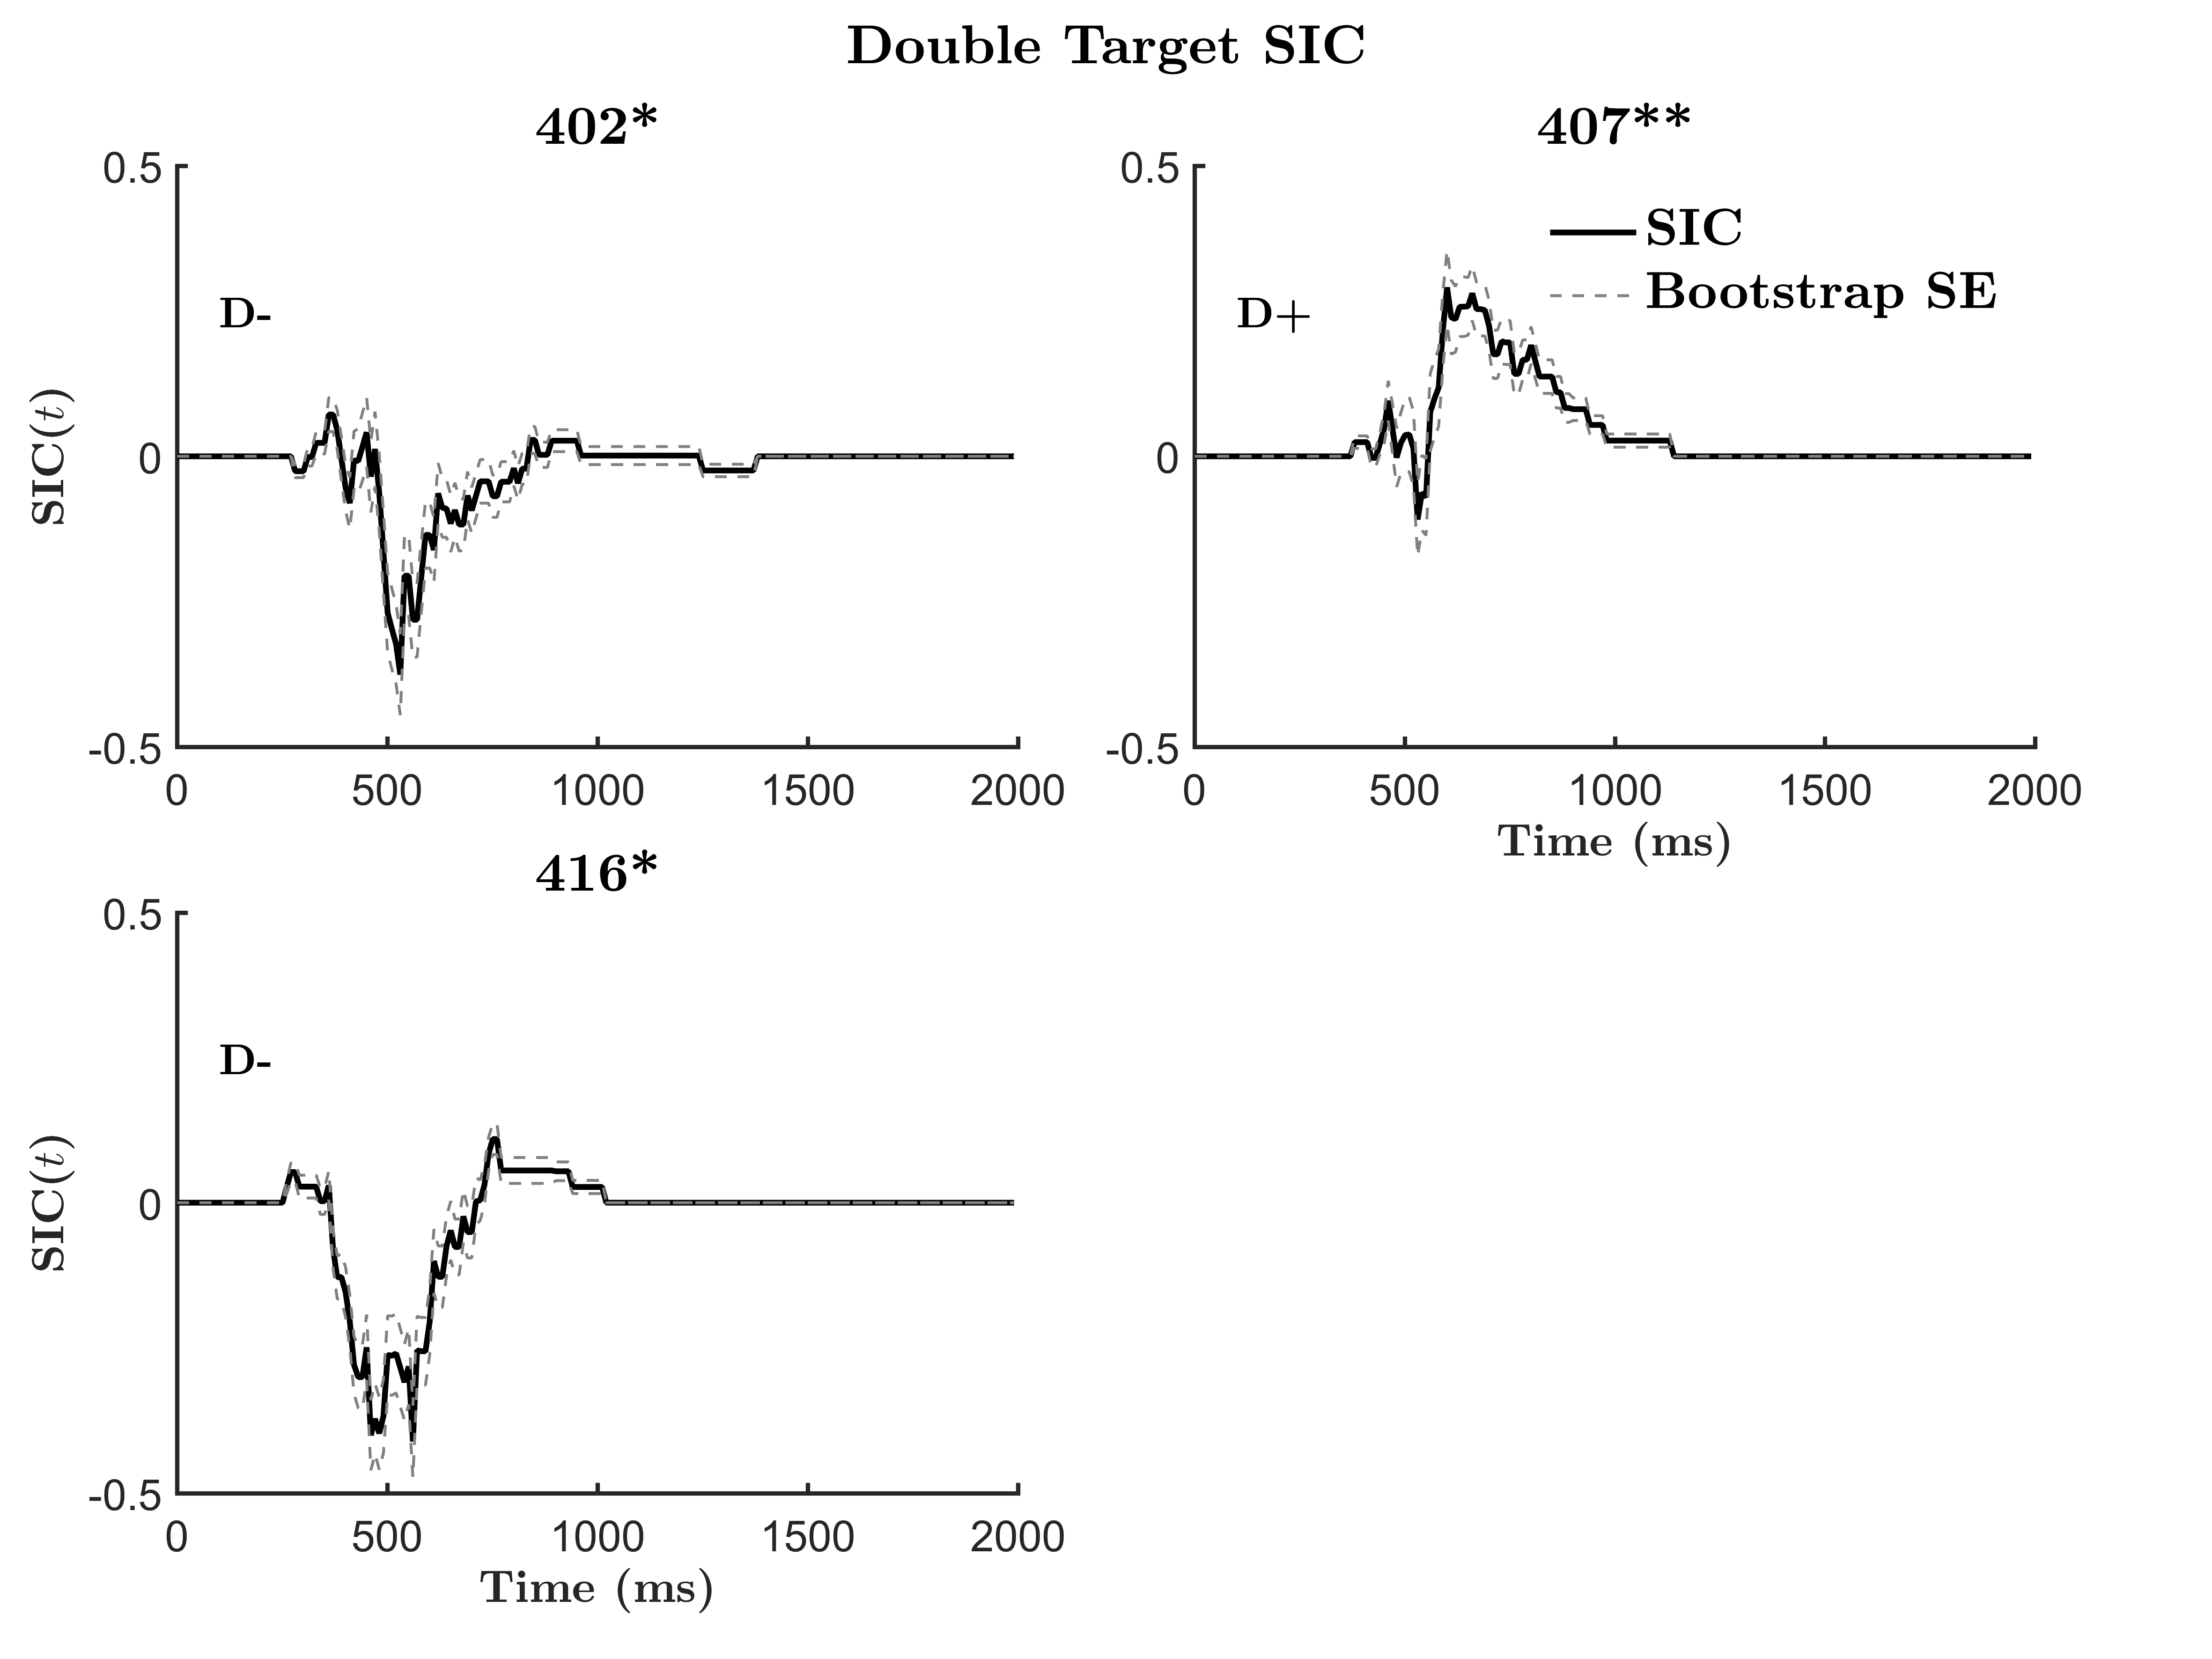
\includegraphics[width=\linewidth]{Figures/Appendix/FIG26PNG.png}
\caption{Double-Target survivor interaction contrast (SIC) plots for each individual subject in Experiment 4. Dotted line illustrates the bootstrap of the standard error.\newline
\textbf{Note.} MIC interaction contrast significance defined at $p$* $<$ .33, $p$** $<$ .05, $p$*** $<$ .01. D-statistic, a measure of SIC deviance from SIC($t$) = 0 significance defined at $\alpha$ $<$ 0.15.}
\label{fig:Indiv_SIC_AB_Ex4}
\end{center}
\end{figure}
\newpage


\section{Individual MIC Plots}
\label{Sup: IndMIC}


\subsection{Experiment 1: Fixed Item-Size, Mixed Item-Sets Double-Target MIC Plots}
\begin{figure}[htb]
\begin{center}
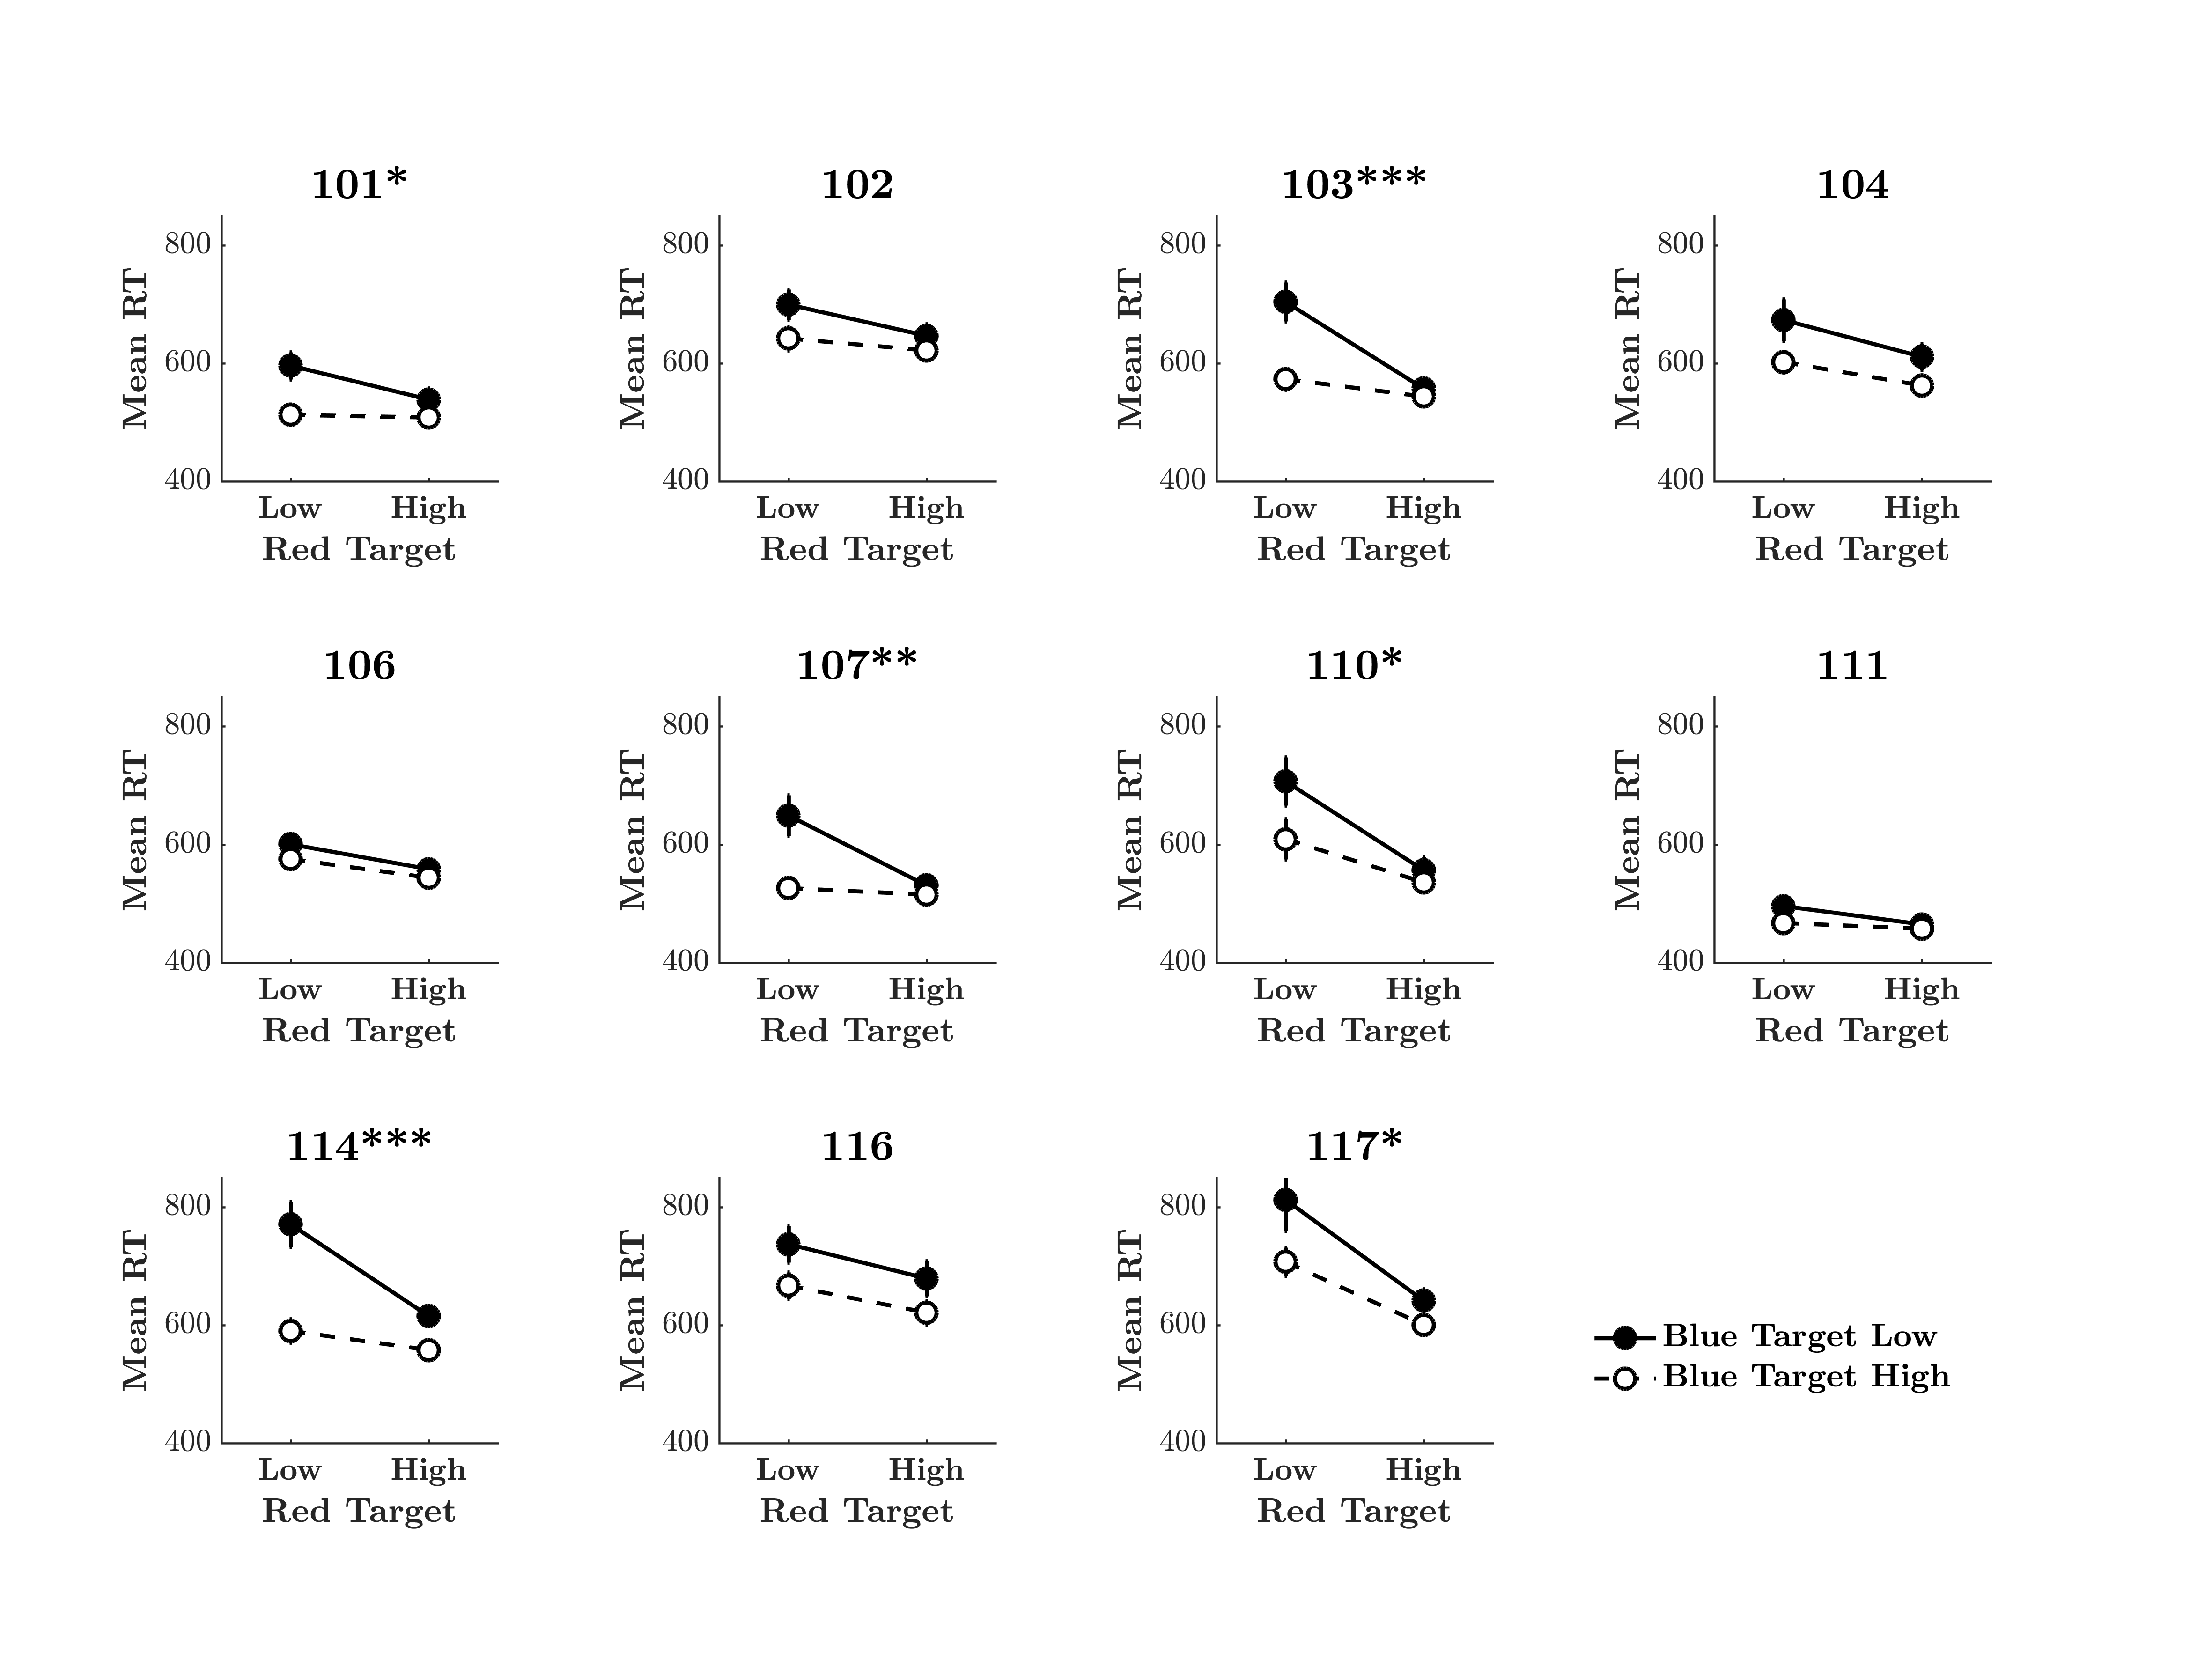
\includegraphics[width=\linewidth]{Figures/Appendix/FIG27PNG.png}
\caption{Double-Target mean interaction contrast (MIC) plots for each individual subject in Experiment 1. White-eggs indicate blue-target high-salience, black-eggs blue-target low-salience. Error bars are $\pm$1 standard error of the mean.  \newline
\textbf{Note.} MIC interaction contrast significance defined at $p$* $<$ .33, $p$** $<$ .05, $p$*** $<$ .01}
\label{fig:Indiv_MIC_AB_Ex1}
\end{center}
\end{figure}
\newpage

\subsection{Experiment 2: Fixed Item-Size, Split Item-Sets Double-Target MIC Plots}
\begin{figure}[htb]
\begin{center}
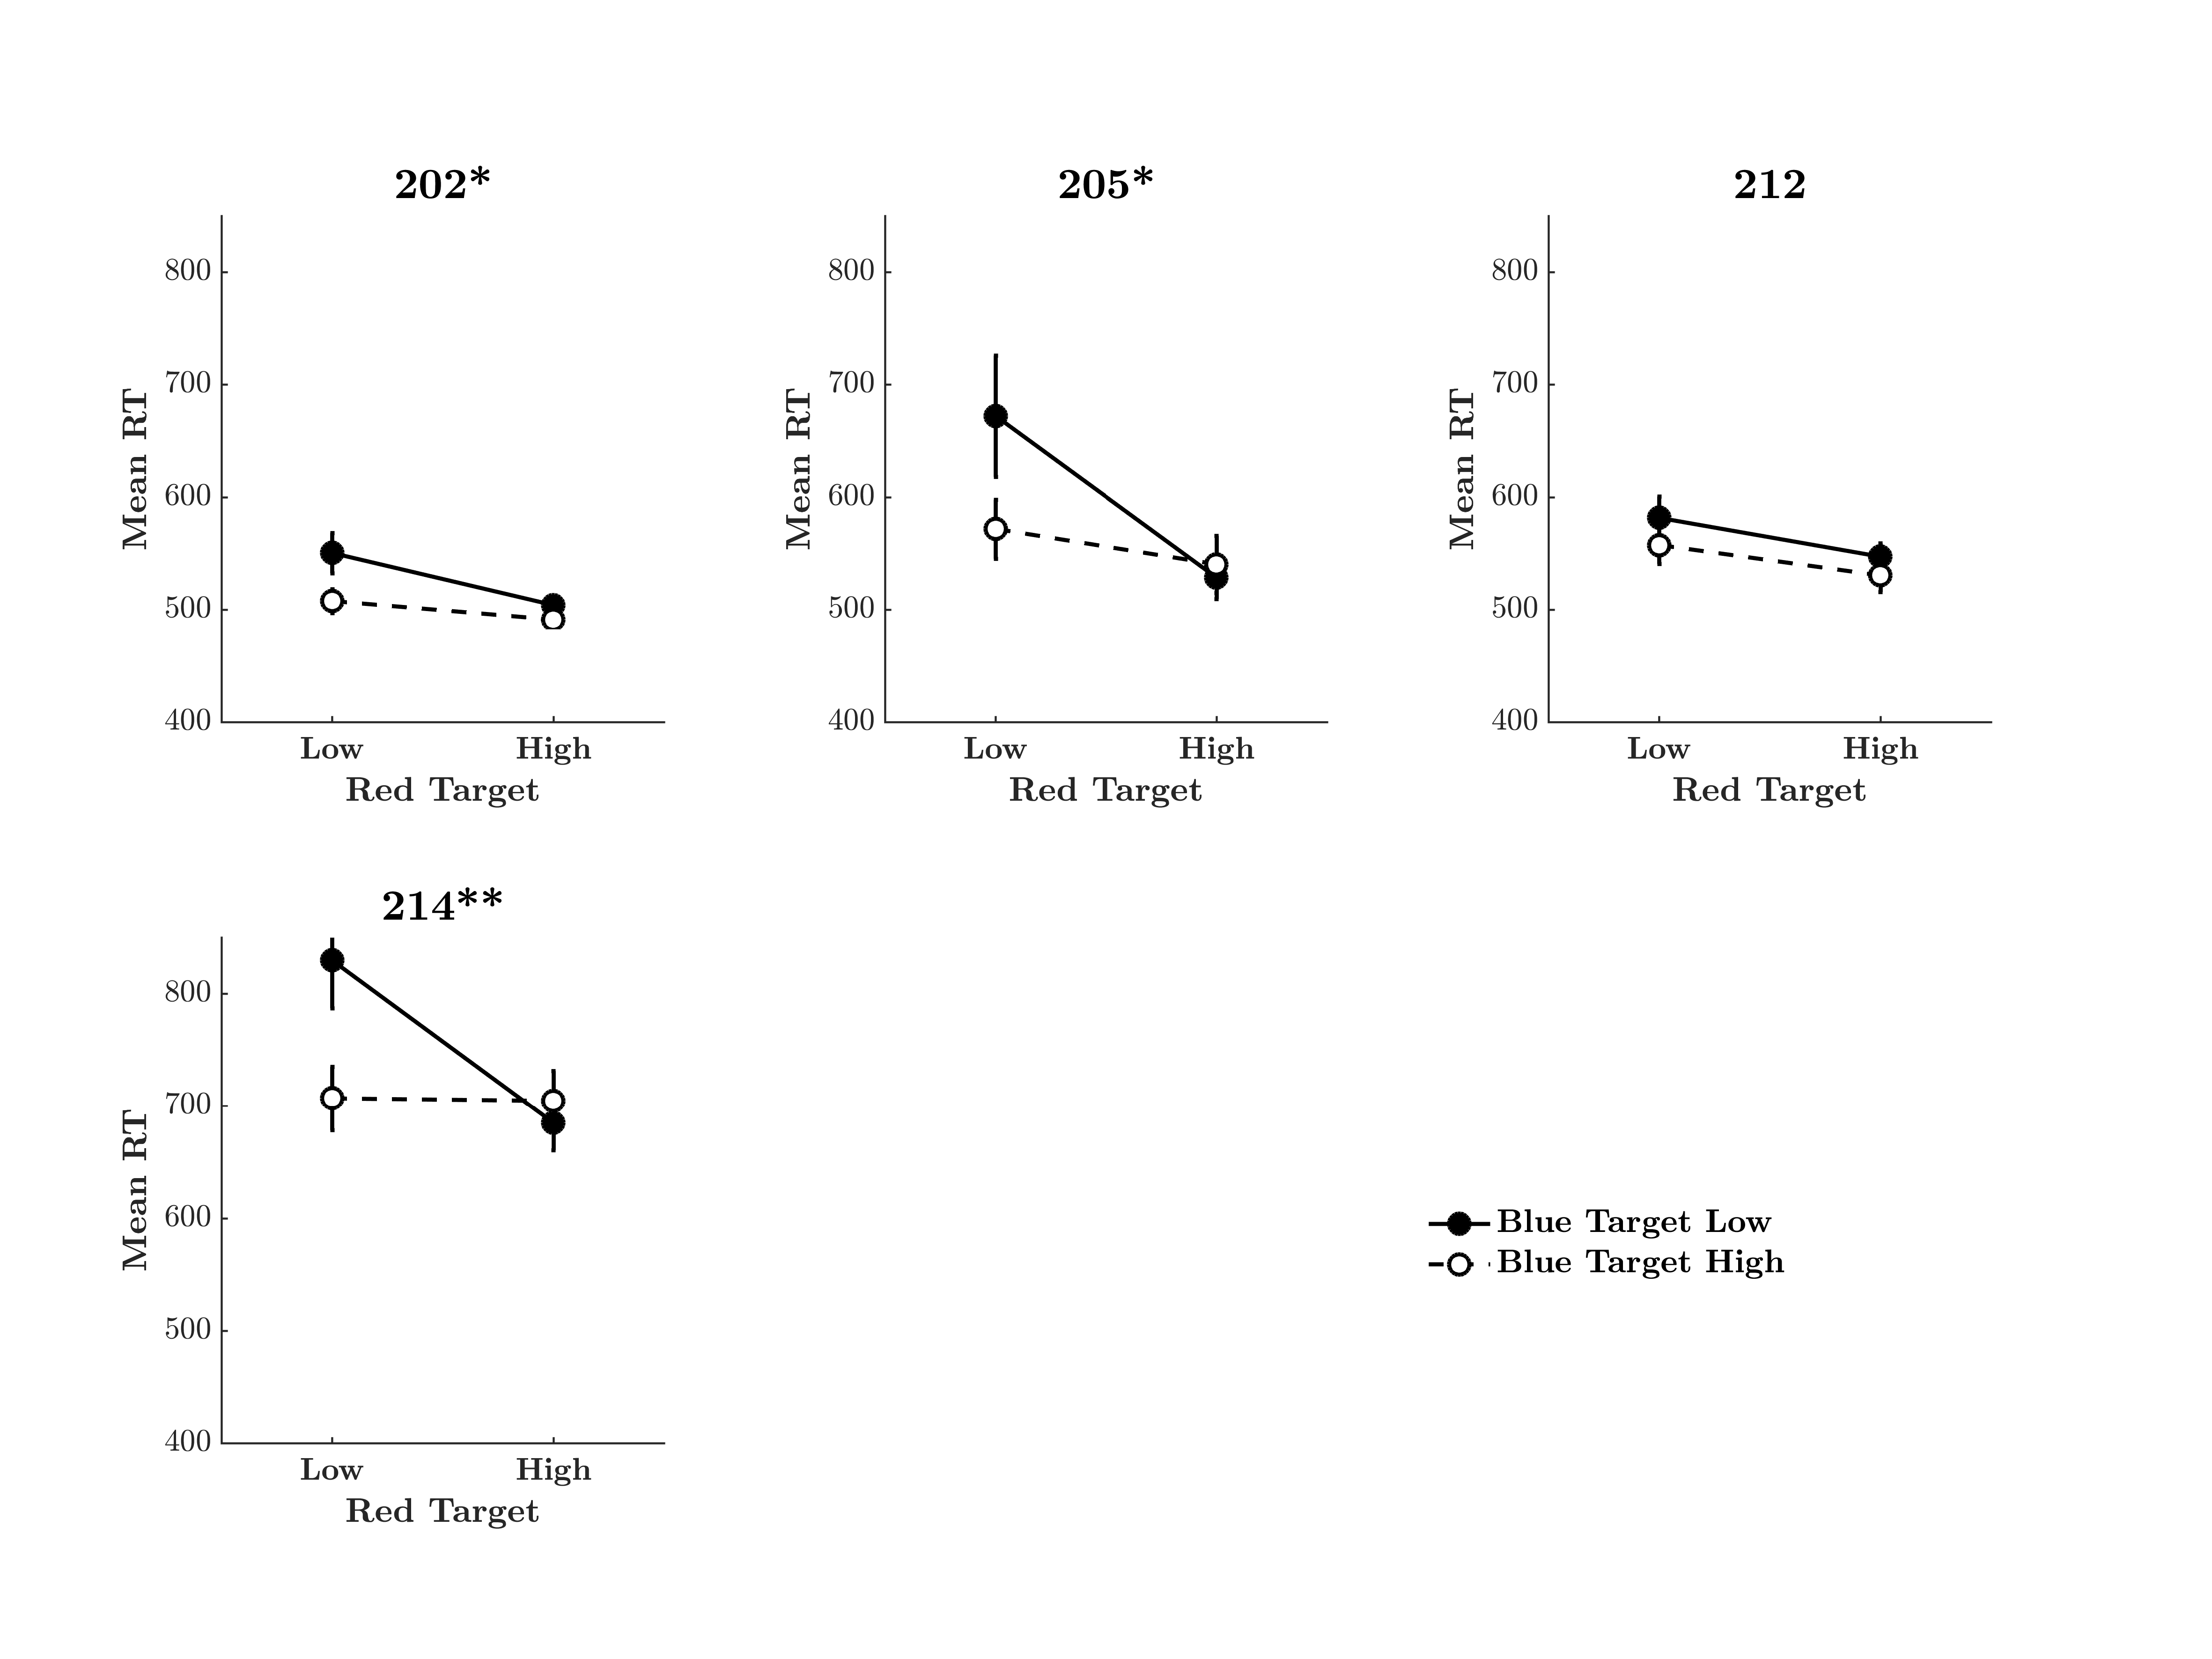
\includegraphics[width=\linewidth]{Figures/Appendix/FIG28PNG.png}
\caption{Double-Target mean interaction contrast (MIC) plots for each individual subject in Experiment 2. White-eggs indicate blue-target high-salience, black-eggs blue-target low-salience. Error bars are $\pm$1 standard error of the mean. \newline
\textbf{Note.} MIC interaction contrast significance defined at $p$* $<$ .33, $p$** $<$ .05, $p$*** $<$ .01}
\label{fig:Indiv_MIC_AB_Ex2}
\end{center}
\end{figure}
\newpage

\subsection{Experiment 3: Fixed Area, Mixed Item-Sets Double-Target MIC Plots}
\begin{figure}[htb]
\begin{center}
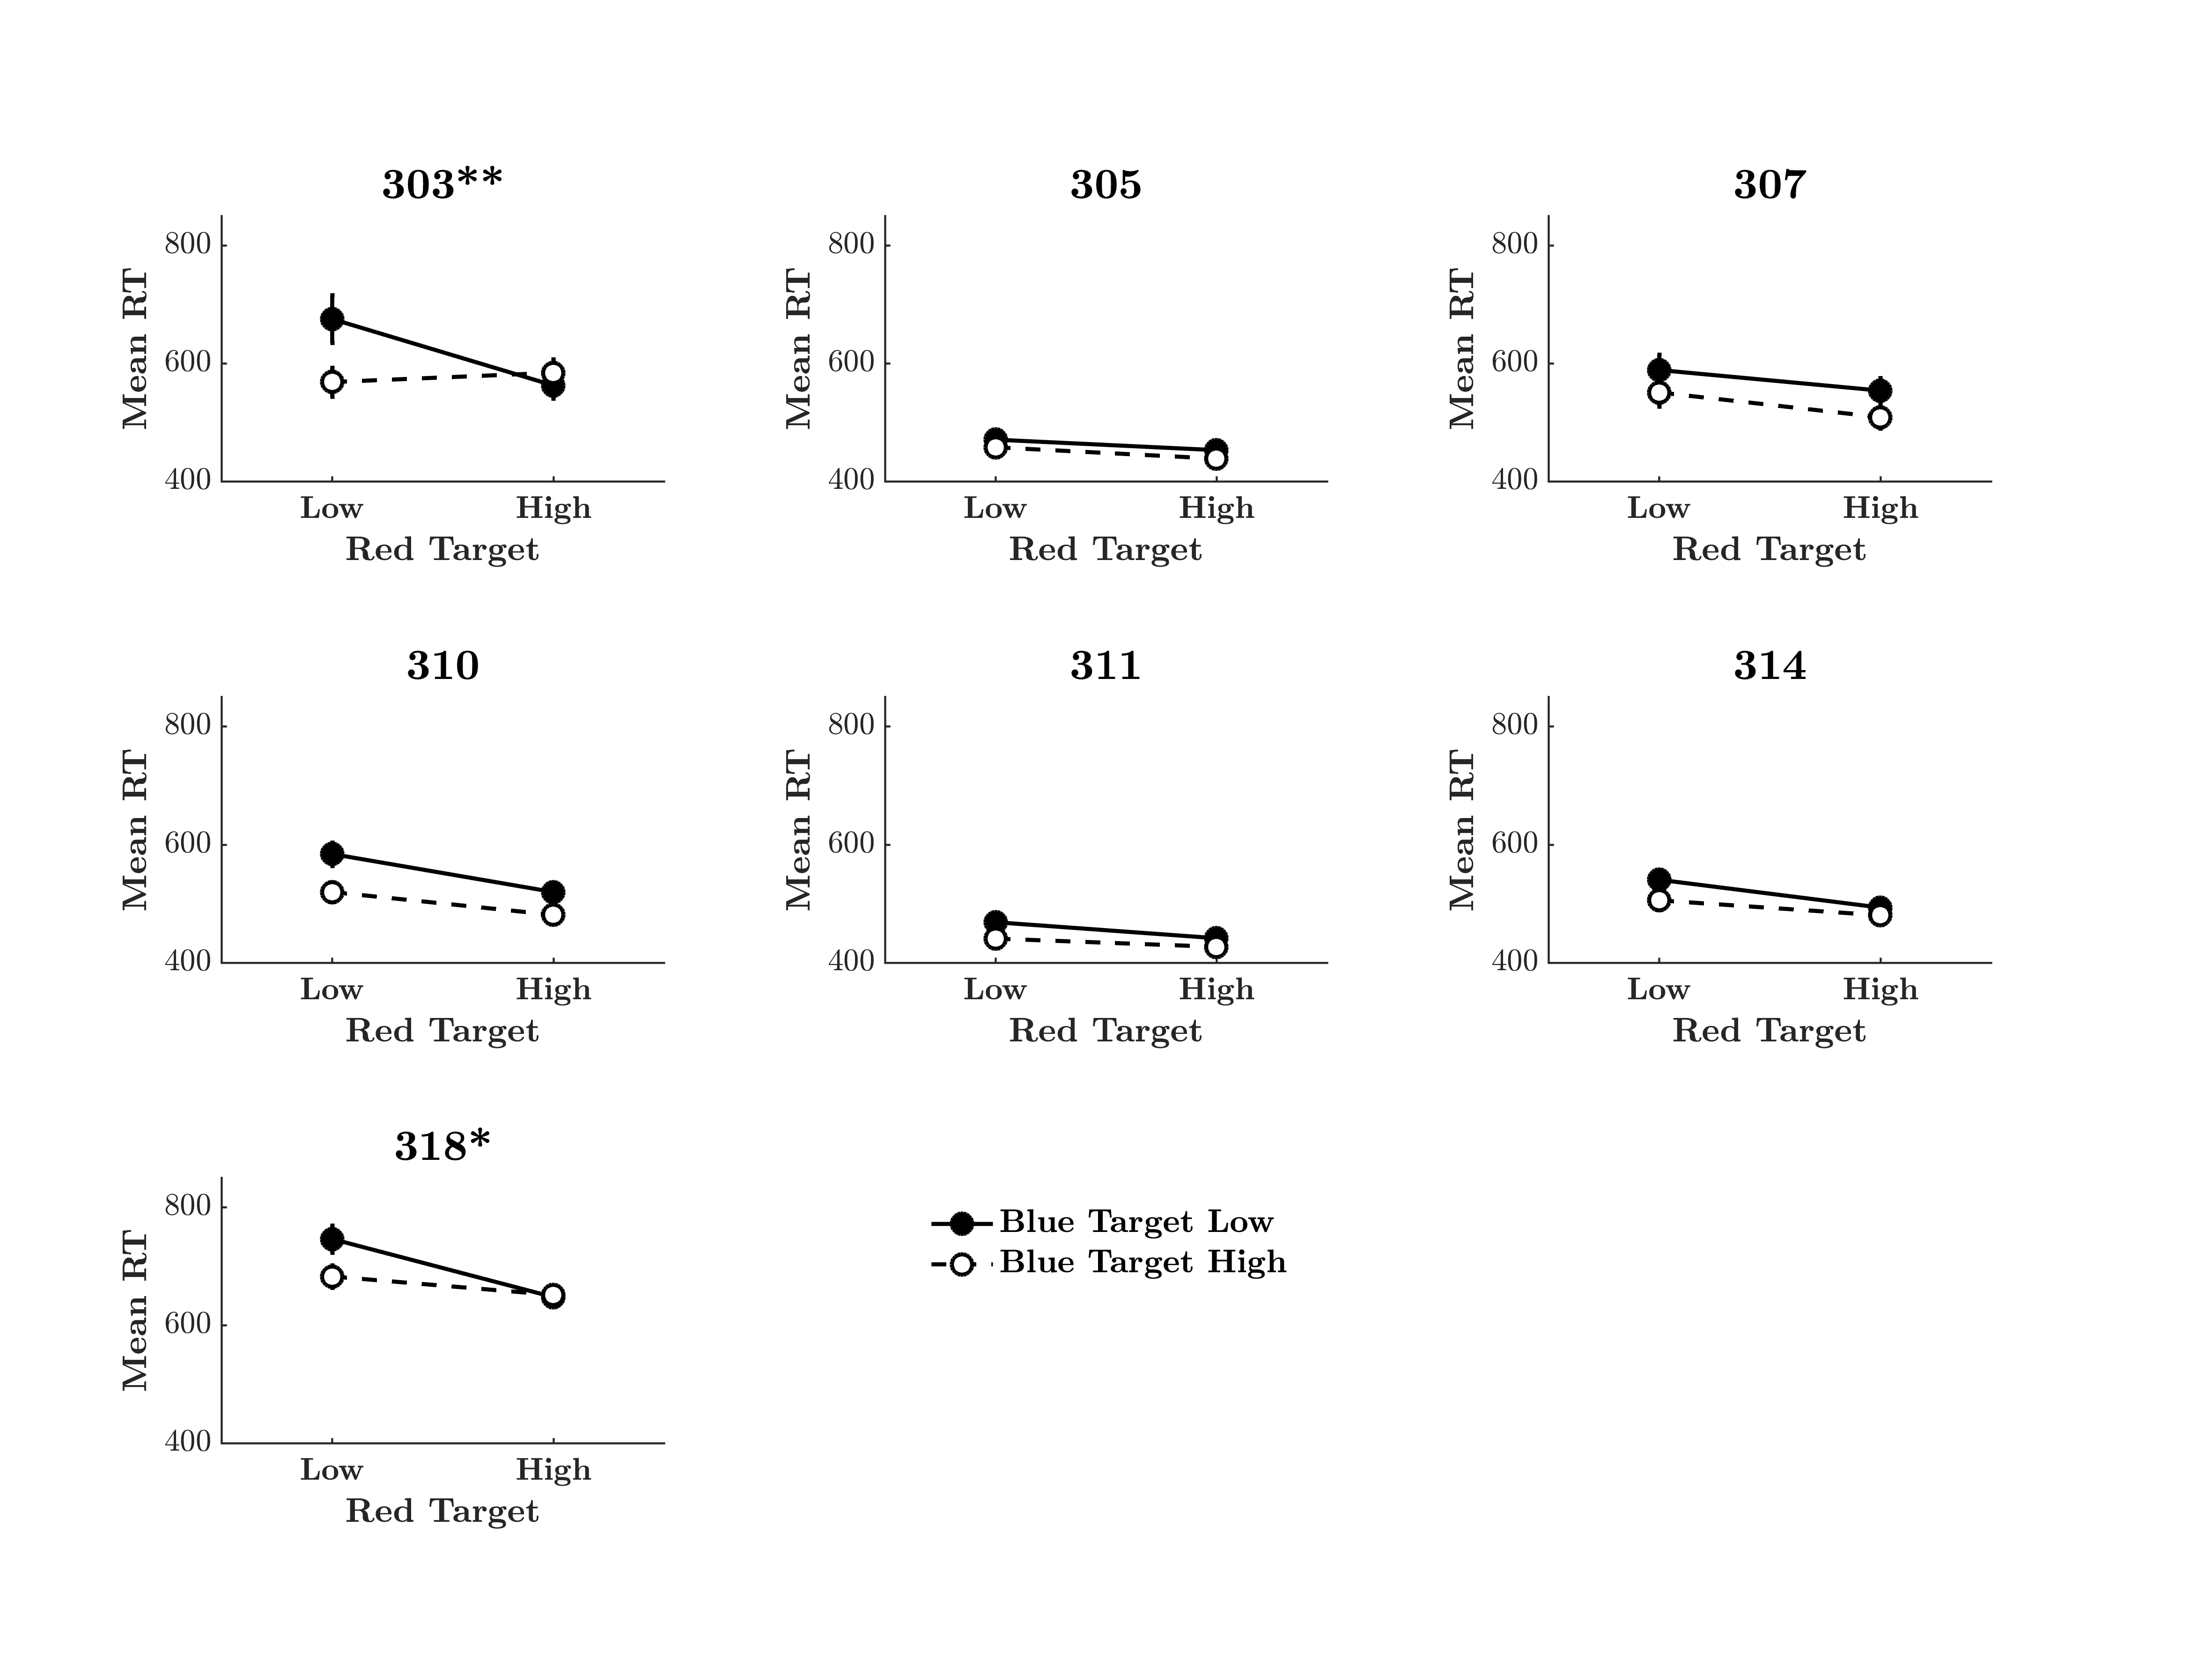
\includegraphics[width=\linewidth]{Figures/Appendix/FIG29PNG.png}
\caption{Double-Target mean interaction contrast (MIC) plots for each individual subject in Experiment 3. White-eggs indicate blue-target high-salience, black-eggs blue-target low-salience. Error bars are $\pm$1 standard error of the mean. \newline
\textbf{Note.} MIC interaction contrast significance defined at $p$* $<$ .33, $p$** $<$ .05, $p$*** $<$ .01}
\label{fig:Indiv_MIC_AB_Ex3}
\end{center}
\end{figure}
\newpage

\subsection{Experiment 4: Fixed Area, Split Item-Sets Double-Target MIC Plots}
\begin{figure}[htb]
\begin{center}
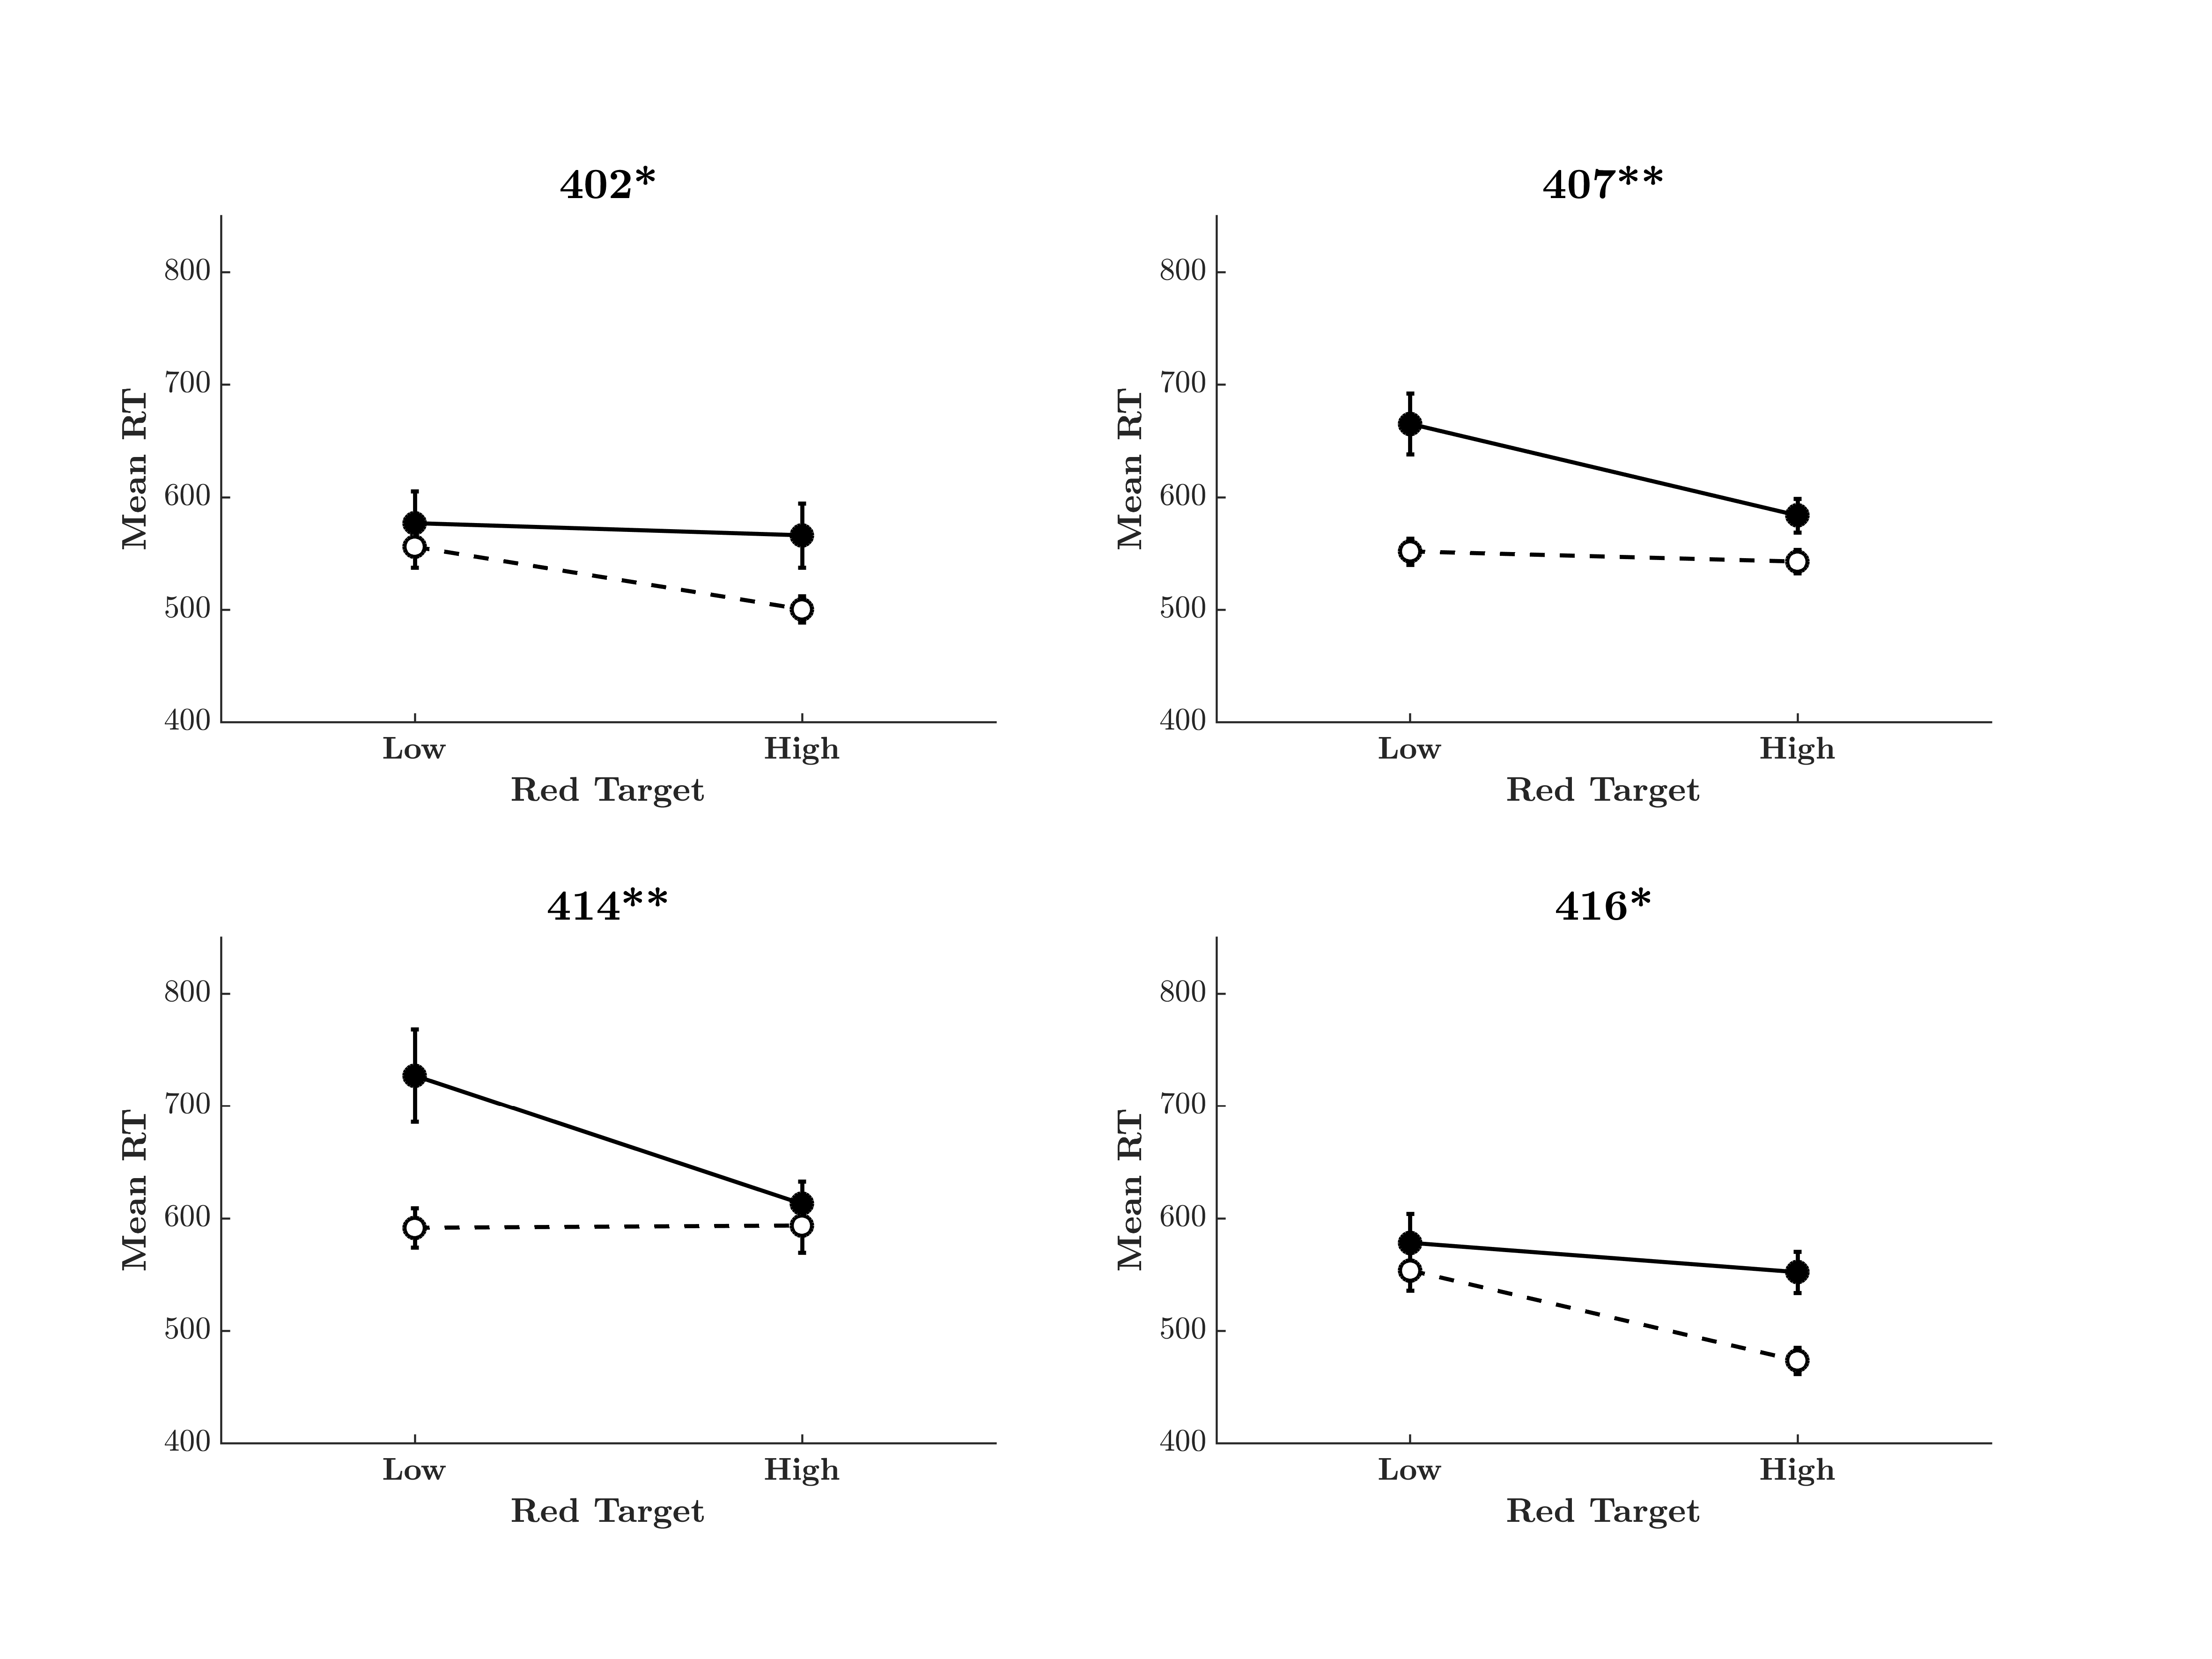
\includegraphics[width=\linewidth]{Figures/Appendix/FIG30PNG.png}
\caption{Double-Target mean interaction contrast (MIC) plots for each individual subject in Experiment 4. White-eggs indicate blue-target high-salience, black-eggs blue-target low-salience. Error bars are $\pm$1 standard error of the mean. \newline
\textbf{Note.} MIC interaction contrast significance defined at $p$* $<$ .33, $p$** $<$ .05, $p$*** $<$ .01}
\label{fig:Indiv_MIC_AB_Ex4}
\end{center}
\end{figure}
\newpage

